% Options for packages loaded elsewhere
\PassOptionsToPackage{unicode}{hyperref}
\PassOptionsToPackage{hyphens}{url}
\documentclass[
]{article}
\usepackage{xcolor}
\usepackage{amsmath,amssymb}
\setcounter{secnumdepth}{5}
\usepackage{iftex}
\ifPDFTeX
  \usepackage[T1]{fontenc}
  \usepackage[utf8]{inputenc}
  \usepackage{textcomp} % provide euro and other symbols
\else % if luatex or xetex
  \usepackage{unicode-math} % this also loads fontspec
  \defaultfontfeatures{Scale=MatchLowercase}
  \defaultfontfeatures[\rmfamily]{Ligatures=TeX,Scale=1}
\fi
% \usepackage{lmodern}
\ifPDFTeX\else
  % xetex/luatex font selection
\fi
% Use upquote if available, for straight quotes in verbatim environments
\IfFileExists{upquote.sty}{\usepackage{upquote}}{}
\IfFileExists{microtype.sty}{% use microtype if available
  \usepackage[]{microtype}
  \UseMicrotypeSet[protrusion]{basicmath} % disable protrusion for tt fonts
}{}
\makeatletter
\@ifundefined{KOMAClassName}{% if non-KOMA class
  \IfFileExists{parskip.sty}{%
    \usepackage{parskip}
  }{% else
    \setlength{\parindent}{0pt}
    \setlength{\parskip}{6pt plus 2pt minus 1pt}}
}{% if KOMA class
  \KOMAoptions{parskip=half}}
\makeatother
\usepackage{longtable,booktabs,array}
\newcounter{none} % for unnumbered tables
\usepackage{calc} % for calculating minipage widths
% Correct order of tables after \paragraph or \subparagraph
\usepackage{etoolbox}
\makeatletter
\patchcmd\longtable{\par}{\if@noskipsec\mbox{}\fi\par}{}{}
\makeatother
% Allow footnotes in longtable head/foot
\IfFileExists{footnotehyper.sty}{\usepackage{footnotehyper}}{\usepackage{footnote}}
\makesavenoteenv{longtable}
\usepackage{graphicx}
\makeatletter
\newsavebox\pandoc@box
\newcommand*\pandocbounded[1]{% scales image to fit in text height/width
  \sbox\pandoc@box{#1}%
  \Gscale@div\@tempa{\textheight}{\dimexpr\ht\pandoc@box+\dp\pandoc@box\relax}%
  \Gscale@div\@tempb{\linewidth}{\wd\pandoc@box}%
  \ifdim\@tempb\p@<\@tempa\p@\let\@tempa\@tempb\fi% select the smaller of both
  \ifdim\@tempa\p@<\p@\scalebox{\@tempa}{\usebox\pandoc@box}%
  \else\usebox{\pandoc@box}%
  \fi%
}
% Set default figure placement to htbp
\def\fps@figure{htbp}
\makeatother
\setlength{\emergencystretch}{3em} % prevent overfull lines
\providecommand{\tightlist}{%
  \setlength{\itemsep}{0pt}\setlength{\parskip}{0pt}}
\usepackage[]{natbib}
\bibliographystyle{plainnat}
\makeatletter
\@ifpackageloaded{subcaption}{}{\usepackage{subcaption}}
\@ifpackageloaded{caption}{}{\usepackage{caption}}
\captionsetup[subfigure]{margin=0.5em}
\AtBeginDocument{%
\renewcommand*\figurename{Figure}
\renewcommand*\tablename{Table}
}
\AtBeginDocument{%
\renewcommand*\listfigurename{List of Figures}
\renewcommand*\listtablename{List of Tables}
}
\newcounter{pandoccrossref@subfigures@footnote@counter}
\newenvironment{pandoccrossrefsubfigures}{%
\setcounter{pandoccrossref@subfigures@footnote@counter}{0}
\begin{figure}\centering%
\gdef\global@pandoccrossref@subfigures@footnotes{}%
\DeclareRobustCommand{\footnote}[1]{\footnotemark%
\stepcounter{pandoccrossref@subfigures@footnote@counter}%
\ifx\global@pandoccrossref@subfigures@footnotes\empty%
\gdef\global@pandoccrossref@subfigures@footnotes{{##1}}%
\else%
\g@addto@macro\global@pandoccrossref@subfigures@footnotes{, {##1}}%
\fi}}%
{\end{figure}%
\addtocounter{footnote}{-\value{pandoccrossref@subfigures@footnote@counter}}
\@for\f:=\global@pandoccrossref@subfigures@footnotes\do{\stepcounter{footnote}\footnotetext{\f}}%
\gdef\global@pandoccrossref@subfigures@footnotes{}}
\@ifpackageloaded{float}{}{\usepackage{float}}
\floatstyle{ruled}
\@ifundefined{c@chapter}{\newfloat{codelisting}{h}{lop}}{\newfloat{codelisting}{h}{lop}[chapter]}
\floatname{codelisting}{Listing}
\newcommand*\listoflistings{\listof{codelisting}{List of Listings}}
\makeatother
\usepackage{bookmark}
\IfFileExists{xurl.sty}{\usepackage{xurl}}{} % add URL line breaks if available
\urlstyle{same}
% fallback for those not using the hyperref driver hyperxmp:
\makeatletter
\@ifundefined{xmpquote}{\newcommand{\xmpquote}[1]{#1}}{}
\makeatother
\hypersetup{
  colorlinks=true,linkcolor=red,urlcolor=red,citecolor=red,anchorcolor=red,filecolor=red,
  pdfcreator={LaTeX via pandoc}}

\author{}
\date{}

\IfFileExists{seqsplit.sty}{\usepackage{seqsplit}}{\newcommand{\seqsplit}[1]{#1}}
\protected\def\breakseq#1{\seqsplit{#1}}
\protected\def\breaktt#1{\begingroup\ttfamily\seqsplit{#1}\endgroup}
\title{Template Madlib: Deterministic Token Injection for Conditional IMRAD Manuscripts}
\author{Daniel Ari Friedman}
\date{2026-06-26}

% Core mathematics
\usepackage{amsmath}
\usepackage{amssymb}
\usepackage{amsfonts}
\usepackage{amsthm}

% Document layout
\usepackage{geometry}
\geometry{margin=0.25in}
\usepackage{float}
\usepackage{graphicx}

% Tables
\usepackage{booktabs}
\usepackage{longtable}
\usepackage{array}

% Algorithm typesetting (for pseudocode in §2 Methodology)
\usepackage[ruled,vlined,linesnumbered]{algorithm2e}

% Code listings
\usepackage{listings}

% Typography and formatting
\usepackage{microtype}
\usepackage{xcolor}
\usepackage[binary-units]{siunitx}

% Cross-references and citations
\usepackage{hyperref}
\hypersetup{
    colorlinks=true,
    allcolors=red
}
\usepackage[capitalise,noabbrev]{cleveref}
\usepackage{natbib}

% ── Unicode-capable mono font for code listings ──────────────────────
% JuliaMono (TeX Live 2026) covers the full math/Greek glyph set used in
% scientific code blocks; the default lmmono lacks \alpha/\mu/\partial/\nabla.
%
% The hardcoded TeX Live 2026 path below is portable to most macOS / Linux
% TeX Live installs that placed JuliaMono under the default texmf-dist path.
% If your TeX Live version differs (e.g., 2025, 2027) or your distribution
% installs fonts elsewhere, comment out the explicit Path = line — fontspec
% will then search the system font path. If JuliaMono is not installed at
% all, comment out the whole block; xelatex falls back to lmmono with
% reduced Unicode coverage but the document still compiles.
\usepackage{fontspec}
\setmonofont{JuliaMono-Regular}[
  Path           = /usr/local/texlive/2026/texmf-dist/fonts/truetype/public/juliamono/,
  Extension      = .ttf,
  UprightFont    = *,
  BoldFont       = JuliaMono-Bold,
  ItalicFont     = JuliaMono-RegularItalic,
  BoldItalicFont = JuliaMono-BoldItalic,
  Scale          = MatchLowercase,
]

% Math font for unicode-math: Latin Modern Math (TeX Live) has full BMP
% coverage including U+2223 (\mid), U+226A/226B (\ll/\gg), and the Greek/
% blackboard letters used in equations. Without an explicit \setmathfont,
% unicode-math falls back to lmroman text font which lacks several glyphs
% and emits "Missing character" warnings on every \mid in math mode.
\setmathfont{latinmodern-math.otf}

\begin{document}

\begin{titlepage}
\centering
\vspace*{0.55cm}
{\Huge\sffamily\bfseries Template Madlib: Deterministic Token Injection for Conditional IMRAD Manuscripts\par}
\vspace{0.4em}
{\Large\sffamily A public exemplar for source-owned lexical composition\par}
\vspace{0.75em}
{\Large\sffamily\bfseries Daniel Ari Friedman\par}
{\normalsize\sffamily Active Inference Institute\par}
{\normalsize\sffamily\texttt{daniel@activeinference.institute}\par}
{\normalsize\sffamily\href{https://orcid.org/0000-0001-6232-9096}{ORCID: 0000-0001-6232-9096}\par}
\vspace{0.18em}
{\normalsize\sffamily DOI: \href{https://doi.org/10.5281/zenodo.20786638}{10.5281/zenodo.20786638}\par}
\vspace{0.35em}
\makeatletter
{\@date\par}
\makeatother
\vfill

\includegraphics[width=0.98\textwidth,height=0.60\textheight,keepaspectratio]{\detokenize{../figures/madlib_cover_overview.png}}
\vfill
\end{titlepage}
\thispagestyle{empty}
\tableofcontents
\newpage


\section{Abstract}\label{abstract}

This exemplar asks whether a reviewable pipeline can hydrate a complete
IMRAD manuscript from configuration-owned lexical data while preserving
an audit trail that remains readable before and after rendering. The
project deliberately keeps playful Mad Lib mechanics inside a serious
reproducibility contract: the manuscript shell names large placeholders,
the config declares allowable language, and the source code decides what
text is emitted.

The committed seed is \texttt{431} and the current schema expands 22
slot rule(s) into 40 token choice(s) across 10 lexicon categories. The
configured narrative moves are state the manuscript-generation problem,
name the deterministic intervention, and summarize the audit surface.
The central hypothesis is: Deterministic lexical injection can generate
a complete conditional IMRAD manuscript while preserving token
provenance, section intent, and audit-ready method evidence.

The result is not a claim that lexical substitution creates scholarship.
It is a worked template for conditional manuscript assembly: section
enablement, token provenance, figure registration, and
unresolved-placeholder checks all become inspectable artifacts before
the shared renderer produces PDF, HTML, and slides.

\newpage

\section{Introduction: Lexicon as Data and Manuscript as Build
Artifact}\label{introduction-lexicon-as-data-and-manuscript-as-build-artifact}

Mad Lib style generation is usually treated as a toy because it
foregrounds the visible blank rather than the source of the replacement.
In a research pipeline, the blank is not the hard part. The hard part is
making every replacement reviewable, deterministic, and honest about
what it can support. \texttt{template\_madlib} turns that constraint
into the subject of the exemplar.

The project treats nouns such as pipeline, protocol, section, lexicon
and verbs such as hydrate, condition, bind, bind as versioned data.
Changing a lexicon entry is therefore closer to changing an input table
than editing prose in place. That distinction matters because the
generated manuscript can be rerendered, diffed, and validated without
asking the reader to trust an invisible drafting session.

The introduction is configured to separate playful Mad Lib syntax from
research claims, identify drift between prose and source data, frame
configuration as an inspectable dataset, and position conditional prose
as a reproducibility problem. Those moves keep the manuscript from
pretending to be an open-ended language model. It is a bounded template:
authors declare categories, slots, section switches, method steps, and
claim boundaries; source code transforms those declarations into
manuscript bodies and evidence tables.

This exemplar is useful for protocols, educational scaffolds, review
forms, templated reports, and other documents where conditional text is
unavoidable but should never become untraceable. The same pattern can be
extended with domain-specific validators while leaving the shared
rendering infrastructure untouched.

\subsection{Contribution Ledger}\label{contribution-ledger}

{\def\LTcaptype{none} % do not increment counter
\begin{longtable}[]{@{}
  >{\raggedright\arraybackslash}p{(\linewidth - 2\tabcolsep) * \real{0.5000}}
  >{\raggedright\arraybackslash}p{(\linewidth - 2\tabcolsep) * \real{0.5000}}@{}}
\toprule\noalign{}
\begin{minipage}[b]{\linewidth}\raggedright
Claim
\end{minipage} & \begin{minipage}[b]{\linewidth}\raggedright
Boundary
\end{minipage} \\
\midrule\noalign{}
\endhead
\bottomrule\noalign{}
\endlastfoot
A Mad Lib manuscript can remain reproducible when the lexicon is treated
as data. & Local exemplar claim; no live DOI or standalone release
implied. \\
Conditional IMRAD section bodies can be rendered without shared renderer
changes. & Local exemplar claim; no live DOI or standalone release
implied. \\
Large-grain manuscript variables can preserve author-readable source
files while still producing a complete manuscript. & Local exemplar
claim; no live DOI or standalone release implied. \\
Token provenance can connect playful lexical substitution to serious
publication hygiene. & Local exemplar claim; no live DOI or standalone
release implied. \\
A generated Methods section can be methodologically useful when protocol
rows, phases, figures, and validation gates share one config-owned
source. & Local exemplar claim; no live DOI or standalone release
implied. \\
Configured-field origin tracking can make loader defaults visible enough
for reviewers and downstream forks. & Local exemplar claim; no live DOI
or standalone release implied. \\
Pipeline-owned output regeneration can keep PDF, HTML, slides, data,
reports, and copied deliverables aligned without hand-editing generated
artifacts. & Local exemplar claim; no live DOI or standalone release
implied. \\
A generated-method exemplar can make review handoff auditable when the
review packet includes source config, data artifacts, figures,
validation results, and copy statistics. & Local exemplar claim; no live
DOI or standalone release implied. \\
Fork migration guidance can reduce overclaiming when it names the
source, test, validator, and evidence surfaces that must change before
domain use. & Local exemplar claim; no live DOI or standalone release
implied. \\
\end{longtable}
}

\newpage

\section{Methods: Source-Owned Token Injection and Conditional IMRAD
Assembly}\label{methods-source-owned-token-injection-and-conditional-imrad-assembly}

The method is conditional section hydration. Each slot combines the
seed, slot name, category, ordinal, and full category list into a
SHA-256 digest; the digest indexes the configured category. Including
the full category list in the digest input means that a lexicon edit can
change the plan in a deterministic and reviewable way instead of
silently preserving stale output.

The deterministic digest recipe is deliberately narrow. It does not
sample from ambient prose, project history, or renderer state; it uses
only the committed seed, the slot declaration, the category name, the
ordinal for repeated slots, and the ordered category inventory. A fork
can therefore explain a changed token choice as a changed seed, slot, or
lexicon row rather than as an opaque generation event.

The first review scenario is declared before generation. The project
names its scope as a local exemplar, records enabled sections, keeps DOI
and publication claims blank, and treats the copy stage as a review
handoff. That ordering matters because a reader should know the allowed
claim boundary before inspecting fluent generated text.

The governing constraint is publication claims stay local until release.
The source manuscript is intentionally sparse: it contains section
titles and large-grain placeholders, not generated claims. The project
script first validates the \texttt{madlib:} block, expands slots into a
\texttt{TokenPlan}, builds section bodies, writes artifact JSON, emits a
figure registry, and only then writes hydrated Markdown under
\breaktt{output/manuscript/}.

The configured method moves are validate config before composition,
declare review scenario and method invariants, separate explicit YAML
fields from loader defaults, govern lexicon categories as reviewable
data, expand slots through seeded digest selection, allocate slot
choices to enabled manuscript sections, compose conditional section
bodies, assemble method evidence tables and visual audit figures, align
generated claims with the claim ledger, emit evidence artifacts before
rendering, verify that no unresolved placeholders remain, assemble a
reviewer packet from regenerated artifacts, and preserve human review
before publication claims. The protocol sequence is Ingest declared
manuscript schema produces \texttt{MadlibConfig}; Declare review
scenario produces \breaktt{review\ scenario}; Track field origin produces
\breaktt{explicit/default\ path\ inventory}; Govern lexicon categories
produces \breaktt{validated\ lexicon}; Construct digest selection
material produces \breaktt{digest\ input\ records}; Record selection
invariants produces \breaktt{selection\ invariant\ set}; Expand slot
declarations produces \texttt{TokenPlan}; Apply section conditions
produces \breaktt{enabled\ section\ set}; Compose conditional IMRAD
bodies produces \breaktt{section\ variables}; Assemble evidence tables
produces \breaktt{Markdown\ evidence\ tables}; Align claims with evidence
ledger produces \breaktt{claim-aligned\ evidence\ surface}; Generate
visual audit surface produces \breaktt{registered\ figure\ set}; Emit
machine-readable artifacts produces
\breaktt{output/data,\ output/reports,\ and\ output/figures}; Hydrate
manuscript shell produces \breaktt{output/manuscript}; Render and
validate deliverables produces \breaktt{validated\ project\ output};
Assemble reviewer packet produces \texttt{review\ packet}; Copy review
surface produces \breaktt{copied\ publication-review\ bundle}; Document
fork migration produces \breaktt{fork\ migration\ notes}. These steps
make the method auditable from three directions: tests inspect the
Python behavior, generated artifacts expose the token plan, and
manuscript validation confirms that no unresolved placeholder survives
into rendered outputs.

The config-origin inventory currently separates 125 explicit YAML
path(s) from 11 loader-defaulted path(s). Treating origin as method
evidence prevents a rendered field from looking equally authored when it
was actually inherited from the loader. The same inventory drives
configured-field tables and figures, so reviewers can inspect which
schema blocks were intentionally set before judging the generated prose.

Method invariants are reviewed as their own artifact. Token choices are
allowed to change when the seed, slot name, category, ordinal, or
ordered category inventory changes; they are not allowed to change
because PDF rendering, HTML rendering, file-copy order, or hand-edited
output changed. This separates generation logic from presentation logic.

Lexicon governance is handled as data governance. Required categories
must be nonempty, optional categories remain project-owned when
declared, and the selected 40 token choice(s) stay bound to 10
configured category list(s). The slot-to-section allocation is abstract:
3, authoring\_contract: 2, configuration: 1, discussion: 3, evaluation:
5, introduction: 8, limitations: 3, methods: 6, reproducibility: 2,
results: 5, scope: 2, which lets the Methods, Results, and provenance
tables state where each lexical decision enters the manuscript.

Conditional section generation is handled before prose assembly. A
disabled section does not vanish and does not borrow claims from an
enabled section; it resolves to an explicit statement that names the
controlling \breaktt{madlib.section\_conditions} key. That behavior keeps
negative or excluded material visible to reviewers.

Evidence tables and visual audit figures are generated from the same
config and \texttt{TokenPlan}. Enabled visualizations are
configured\_field\_matrix, section\_configuration\_heatmap,
field\_origin\_summary, token\_injection\_flow,
section\_token\_allocation, provenance\_trace\_map,
quality\_gate\_matrix; they summarize field origin, token density,
injection flow, section allocation, provenance, and quality gates
without adding independent claims. Figure registration is therefore a
method step: every manuscript image has to be written, registered, and
validated as part of the reproducible render path.

Claim-ledger alignment is part of composition. The contribution table
can make local method claims, but publication, empirical,
reader-quality, and domain-specific claims must either point to evidence
or remain explicit non-claims. This is why the claim ledger, audit
rules, limitations, and authoring contract are generated beside the
Methods rather than written after the fact.

Evaluation is part of the method rather than an afterthought. The config
declares quality probes (Method row completeness, Field-origin
visibility, Placeholder survival, Provenance completeness,
Section-switch observability, Figure registry coverage, Method-figure
alignment, Evidence cleanliness, Fork readiness, Copied-output parity,
Digest invariant review, Claim-ledger alignment, Review packet
completeness, Fork migration sufficiency) and failure modes (Unresolved
placeholder, Overclaimed generated prose, Config-source drift, Figure
provenance gap, Domain misuse, Method row drift, Field-origin opacity,
Visual-method mismatch, Fork without validators, Digest invariant drift,
Claim ledger omission, Review packet incompleteness, Fork migration
ambiguity); the source turns them into tables and validation checks the
rendered surface. That means methods, results, evaluation, and
limitations all share one source-owned schema instead of drifting as
independent prose.

The method is organized around design principles: Configuration owns
prose choices, Method surface is config-owned, Token choice is
deterministic, Field origin is evidence, Sections are conditional but
visible, Visual audit follows data, Generated output is disposable,
Claim boundaries travel with prose, Forks must add validators,
Invariants precede rendering, Diffs are review objects, Review packet is
a method artifact, Fork migration is part of the method. These
principles prevent the Mad Lib surface from becoming a hidden authoring
channel. They require the visible manuscript to stay downstream of
declared inputs, the generated outputs to remain disposable, and the
audit surface to be broad enough for a reviewer to reconstruct how a
sentence reached the PDF.

The operational phases are Schema intake maps
\breaktt{manuscript/config.yaml} to \texttt{MadlibConfig}; Scenario
declaration maps \texttt{MadlibConfig} to \breaktt{review\ scenario};
Field-origin inventory maps \breaktt{MadlibConfig\ and\ raw\ YAML\ keys}
to \breaktt{configured\_field\_inventory.json}; Lexicon validation maps
\breaktt{madlib.lexicon\ and\ madlib.slots} to
\breaktt{validated\ slot\ inventory}; Digest token planning maps
\texttt{MadlibConfig} to \texttt{TokenPlan}; Invariant review maps
\breaktt{TokenPlan\ and\ method\ protocol} to
\breaktt{selection\ invariant\ set}; Slot-to-section allocation maps
\texttt{TokenPlan} to \breaktt{section\ token\ counts}; Section
composition maps \breaktt{TokenPlan\ and\ narrative\ moves} to
\breaktt{manuscript\ variable\ map}; Evidence table assembly maps
\breaktt{MadlibConfig\ and\ TokenPlan} to
\breaktt{manuscript\_variables.json}; Claim-ledger alignment maps
\breaktt{MadlibConfig,\ generated\ prose,\ and\ data/claim\_ledger.yaml}
to \breaktt{claim-aligned\ evidence\ surface}; Visualization emission
maps
\breaktt{MadlibConfig,\ TokenPlan,\ and\ configured-field\ inventory} to
\breaktt{output/figures\ and\ figure\_registry.json}; Artifact emission
maps \breaktt{MadlibConfig\ and\ TokenPlan} to
\breaktt{output/data,\ output/reports,\ and\ output/figures}; Manuscript
hydration maps
\breaktt{source\ manuscript\ shells\ and\ manuscript\_variables.json} to
\breaktt{hydrated\ Markdown\ manuscript}; Render maps
\breaktt{output/manuscript} to
\breaktt{output/pdf,\ output/web,\ and\ output/slides}; Validate and copy
maps \breaktt{project\ output\ directories} to
\breaktt{output/templates/template\_madlib}; Review packet assembly maps
\breaktt{validated\ project\ output\ and\ copy\ statistics} to
\texttt{review\ packet}; Fork contract documentation maps
\breaktt{source\ docs,\ authoring\ contract,\ and\ claim\ ledger} to
\breaktt{fork\ migration\ notes}. Each phase has an explicit input,
transformation, output, and guard. This makes the pipeline explainable
at manuscript scale: a reader can follow the path from YAML declarations
to token choices, from token choices to section bodies, from section
bodies to rendered artifacts, and from rendered artifacts to validation
reports.

The reviewer packet is also a method artifact. The handoff surface is
hydrated Markdown, combined PDF, web output, slides, figures, data JSON,
reports, validation results, and copy statistics; a PDF alone is
insufficient because it cannot show the token inventory, field-origin
inventory, figure registry, validation report, or copied-output
statistics. The declared authoring obligations are Review generated
claims, Review config diffs, Extend claim evidence, Add domain
validators, Rerun the full project path, Review method invariants,
Assemble reviewer packet, Write fork migration notes, which convert that
packet into review work a human can actually perform.

The claim-boundary contract is also generated. The audit-rule list
contains 12 rule(s), and the contribution table binds each local claim
to a non-publication boundary. The final copy stage is a human-review
handoff, not proof that the Mad Lib surface is empirically valid or
ready for a standalone release.

Fork migration closes the method. A downstream project should update
config rows, source-owned composition, validators, claim-ledger entries,
and documentation before replacing exemplar vocabulary with domain
claims. Without that migration work, the fork has only changed words,
not the evidential status of the generated manuscript.

\begin{figure}
\centering
\pandocbounded{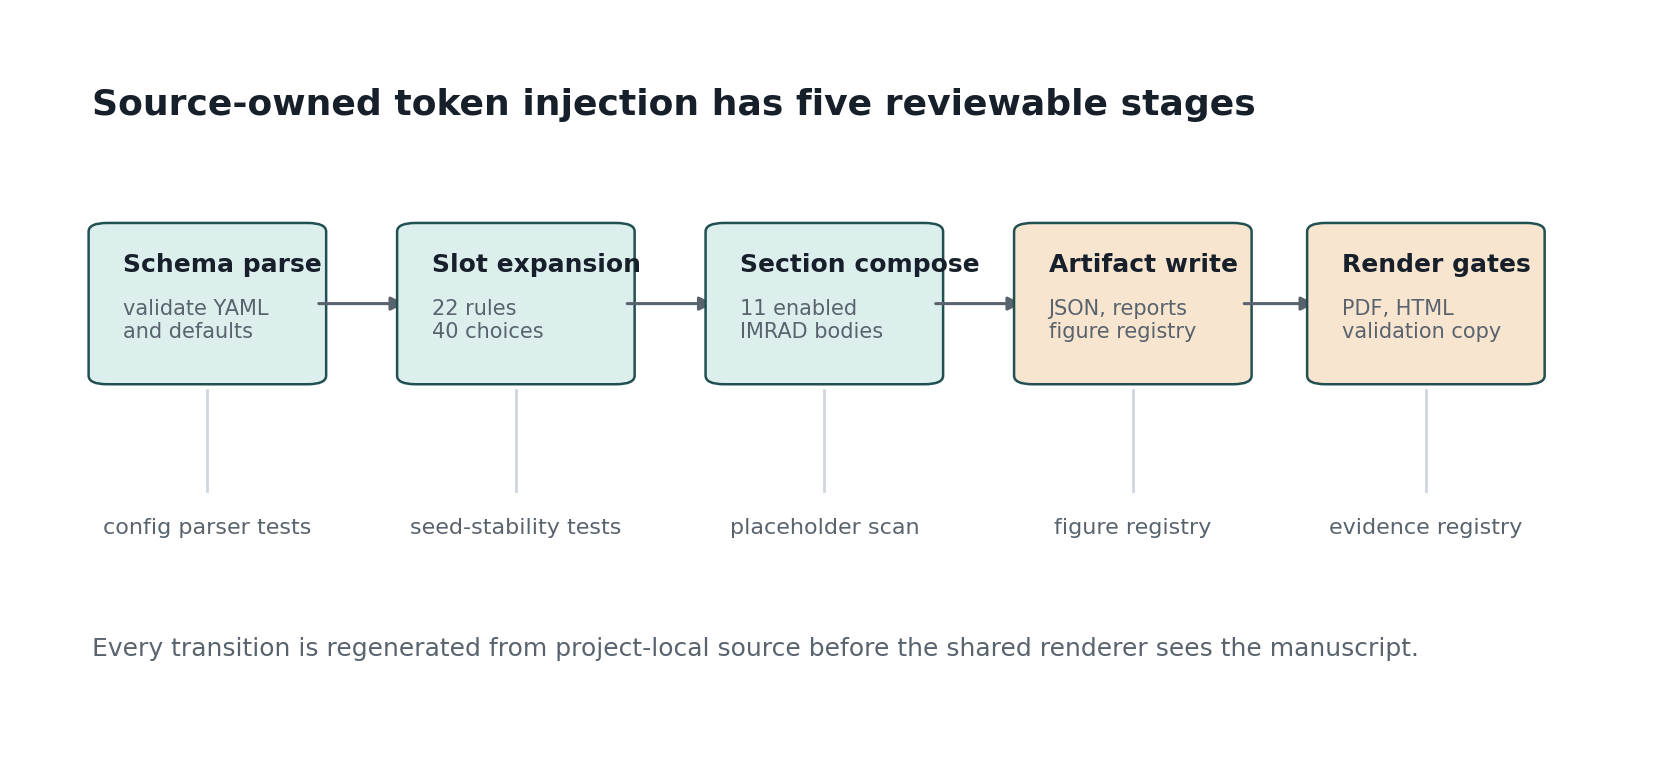
\includegraphics[keepaspectratio,alt={Deterministic token-injection flow}]{../figures/token_injection_flow.png}}
\caption{Deterministic token-injection
flow}\label{fig:token-injection-flow}
\end{figure}

\subsection{Design Principles}\label{design-principles}

{\def\LTcaptype{none} % do not increment counter
\begin{longtable}[]{@{}
  >{\raggedright\arraybackslash}p{(\linewidth - 4\tabcolsep) * \real{0.3333}}
  >{\raggedright\arraybackslash}p{(\linewidth - 4\tabcolsep) * \real{0.3333}}
  >{\raggedright\arraybackslash}p{(\linewidth - 4\tabcolsep) * \real{0.3333}}@{}}
\toprule\noalign{}
\begin{minipage}[b]{\linewidth}\raggedright
Principle
\end{minipage} & \begin{minipage}[b]{\linewidth}\raggedright
Rationale
\end{minipage} & \begin{minipage}[b]{\linewidth}\raggedright
Manuscript effect
\end{minipage} \\
\midrule\noalign{}
\endhead
\bottomrule\noalign{}
\endlastfoot
Configuration owns prose choices & Reviewers can inspect the declared
language surface before generation. & Large-grain manuscript variables
are generated from YAML and project source. \\
Method surface is config-owned & A fork should change method protocol
rows before changing generated Methods prose. & The Methods tables and
body summarize method\_protocol and pipeline\_phases from YAML. \\
Token choice is deterministic & A fixed seed and lexicon must produce
the same injection plan across reruns. & Token inventory rows can be
regenerated and diffed. \\
Field origin is evidence & A generated manuscript should distinguish
authored YAML fields from loader defaults. & Configured-field tables and
figures report explicit and defaulted paths. \\
Sections are conditional but visible & Disabled material should be
auditable rather than silently absent. & Every disabled section resolves
to an explicit disabled-section body. \\
Visual audit follows data & Figures should explain the generated method
without becoming decorative claims. & Cover, flow, allocation,
provenance, gate, and field-origin figures are regenerated from
artifacts. \\
Generated output is disposable & The durable artifact is the
regeneration contract, not hand-edited output files. & Output Markdown,
PDF, HTML, and slides are rebuilt from source inputs. \\
Claim boundaries travel with prose & Generated text can otherwise imply
validation that no artifact supports. & Contribution, limitation,
failure-mode, and authoring tables carry boundary text. \\
Forks must add validators & Domain claims need domain evidence beyond
this exemplar's generic regeneration gates. & Scope, limitations, and
authoring contract require validators before domain claims. \\
Invariants precede rendering & Readers need to know which inputs are
allowed to alter generated tokens before they inspect output. & Methods
names the digest inputs and excludes renderer state from token
choice. \\
Diffs are review objects & Config, token inventory, manuscript
variables, figures, and copied outputs should be diffable review
surfaces. & Methods and reproducibility text describe review packet
assembly after regeneration. \\
Review packet is a method artifact & A PDF alone is insufficient
evidence for a generated-method exemplar. & Authoring contract and
validation sections treat data, reports, figures, and logs as part of
review. \\
Fork migration is part of the method & A public exemplar should teach
authors what must change before domain use. & Standalone notes,
authoring obligations, and claim-ledger boundaries name fork
responsibilities. \\
\end{longtable}
}

\subsection{Operational Phases}\label{operational-phases}

{\def\LTcaptype{none} % do not increment counter
\begin{longtable}[]{@{}
  >{\raggedright\arraybackslash}p{(\linewidth - 8\tabcolsep) * \real{0.2000}}
  >{\raggedright\arraybackslash}p{(\linewidth - 8\tabcolsep) * \real{0.2000}}
  >{\raggedright\arraybackslash}p{(\linewidth - 8\tabcolsep) * \real{0.2000}}
  >{\raggedright\arraybackslash}p{(\linewidth - 8\tabcolsep) * \real{0.2000}}
  >{\raggedright\arraybackslash}p{(\linewidth - 8\tabcolsep) * \real{0.2000}}@{}}
\toprule\noalign{}
\begin{minipage}[b]{\linewidth}\raggedright
Phase
\end{minipage} & \begin{minipage}[b]{\linewidth}\raggedright
Input
\end{minipage} & \begin{minipage}[b]{\linewidth}\raggedright
Transformation
\end{minipage} & \begin{minipage}[b]{\linewidth}\raggedright
Output
\end{minipage} & \begin{minipage}[b]{\linewidth}\raggedright
Guard
\end{minipage} \\
\midrule\noalign{}
\endhead
\bottomrule\noalign{}
\endlastfoot
Schema intake & \breaktt{manuscript/config.yaml} & Load paper metadata
and validate the madlib schema before generation. &
\texttt{MadlibConfig} & config parser tests \\
Scenario declaration & \texttt{MadlibConfig} & Summarize local scope,
enabled sections, claim boundaries, and review handoff expectations. &
\breaktt{review\ scenario} & method protocol and contribution table
tests \\
Field-origin inventory & \breaktt{MadlibConfig\ and\ raw\ YAML\ keys} &
Classify supported paths as explicit or defaulted. &
\breaktt{configured\_field\_inventory.json} & configured-field inventory
tests \\
Lexicon validation & \breaktt{madlib.lexicon\ and\ madlib.slots} & Reject
empty required categories and slot references to missing categories. &
\breaktt{validated\ slot\ inventory} & malformed-config tests \\
Digest token planning & \texttt{MadlibConfig} & Hash seed, slot name,
category, ordinal, and category inventory. & \texttt{TokenPlan} &
seed-stability tests \\
Invariant review & \breaktt{TokenPlan\ and\ method\ protocol} & Confirm
allowed token-choice inputs are documented and isolated from renderer
state. & \breaktt{selection\ invariant\ set} & token determinism and
Methods prose tests \\
Slot-to-section allocation & \texttt{TokenPlan} & Assign each selected
token to its configured manuscript section. &
\breaktt{section\ token\ counts} & provenance and allocation tests \\
Section composition & \breaktt{TokenPlan\ and\ narrative\ moves} & Build
conditional section bodies, titles, and evidence tables. &
\breaktt{manuscript\ variable\ map} & placeholder-coverage tests \\
Evidence table assembly & \breaktt{MadlibConfig\ and\ TokenPlan} & Render
protocol, phase, audit, token, section, provenance, and configured-field
tables. & \breaktt{manuscript\_variables.json} & composition table
tests \\
Claim-ledger alignment &
\breaktt{MadlibConfig,\ generated\ prose,\ and\ data/claim\_ledger.yaml}
& Check local claims and non-claims against source-owned evidence rows.
& \breaktt{claim-aligned\ evidence\ surface} & claim ledger and evidence
registry review \\
Visualization emission &
\breaktt{MadlibConfig,\ TokenPlan,\ and\ configured-field\ inventory} &
Generate cover, flow, allocation, provenance, gate, and configured-field
figures. & \breaktt{output/figures\ and\ figure\_registry.json} &
nonblank figure tests \\
Artifact emission & \breaktt{MadlibConfig\ and\ TokenPlan} & Write
inventory, section plan, injection trace, summary, cover overview,
manuscript figures, and registry. &
\breaktt{output/data,\ output/reports,\ and\ output/figures} &
artifact-writing tests \\
Manuscript hydration &
\breaktt{source\ manuscript\ shells\ and\ manuscript\_variables.json} &
Resolve large-grain placeholders into output/manuscript. &
\breaktt{hydrated\ Markdown\ manuscript} & unresolved-token scan \\
Render & \breaktt{output/manuscript} & Render PDF, HTML, and slides
through the shared template pipeline. &
\breaktt{output/pdf,\ output/web,\ and\ output/slides} & render
command \\
Validate and copy & \breaktt{project\ output\ directories} & Validate
files, registries, evidence, overlays, and copied deliverables. &
\breaktt{output/templates/template\_madlib} & validation and copy
commands \\
Review packet assembly &
\breaktt{validated\ project\ output\ and\ copy\ statistics} & Group
manuscript, web, slides, figures, data, reports, validation results, and
copy statistics as the review surface. & \texttt{review\ packet} &
copied-output validation \\
Fork contract documentation &
\breaktt{source\ docs,\ authoring\ contract,\ and\ claim\ ledger} & State
which config, source, test, validator, and evidence surfaces a fork must
change before domain claims. & \breaktt{fork\ migration\ notes} &
documentation and claim-ledger tests \\
\end{longtable}
}

\subsection{Protocol Steps}\label{protocol-steps}

{\def\LTcaptype{none} % do not increment counter
\begin{longtable}[]{@{}
  >{\raggedright\arraybackslash}p{(\linewidth - 6\tabcolsep) * \real{0.2500}}
  >{\raggedright\arraybackslash}p{(\linewidth - 6\tabcolsep) * \real{0.2500}}
  >{\raggedright\arraybackslash}p{(\linewidth - 6\tabcolsep) * \real{0.2500}}
  >{\raggedright\arraybackslash}p{(\linewidth - 6\tabcolsep) * \real{0.2500}}@{}}
\toprule\noalign{}
\begin{minipage}[b]{\linewidth}\raggedright
Step
\end{minipage} & \begin{minipage}[b]{\linewidth}\raggedright
Action
\end{minipage} & \begin{minipage}[b]{\linewidth}\raggedright
Evidence
\end{minipage} & \begin{minipage}[b]{\linewidth}\raggedright
Output
\end{minipage} \\
\midrule\noalign{}
\endhead
\bottomrule\noalign{}
\endlastfoot
Ingest declared manuscript schema & Parse paper metadata and the madlib
block from manuscript/config.yaml before any prose or figures are
composed. & Config validation tests and MadlibConfig construction from
the committed YAML. & \texttt{MadlibConfig} \\
Declare review scenario & Name the manuscript scope, local claim
boundary, enabled sections, and intended reviewer handoff before token
generation. & section\_plan.json, contribution table, and authoring
contract rows. & \breaktt{review\ scenario} \\
Track field origin & Record every supported madlib path as explicit when
it appears in YAML or defaulted when the loader supplies it. &
configured\_field\_inventory.json and configured-field origin tests. &
\breaktt{explicit/default\ path\ inventory} \\
Govern lexicon categories & Reject empty required categories, preserve
project-owned optional categories, and treat every lexical list as
source data. & Malformed-config tests and lexicon rows in
token\_inventory.json. & \breaktt{validated\ lexicon} \\
Construct digest selection material & Combine seed, slot name, category,
ordinal, and the full category inventory into a deterministic digest
input. & Seed-stability and category-sensitivity tests. &
\breaktt{digest\ input\ records} \\
Record selection invariants & State the invariant inputs that are
allowed to change token choices and the renderer state that is not
allowed to affect them. & Token determinism tests and Methods digest
prose. & \breaktt{selection\ invariant\ set} \\
Expand slot declarations & Resolve every slot count into one or more
token choices and assign each selected value to its configured
manuscript section. & TokenPlan construction, provenance trace, and
section allocation figure. & \texttt{TokenPlan} \\
Apply section conditions & Evaluate section switches before prose
assembly so disabled sections receive explicit disabled-section bodies.
& Section-condition tests and output/data/section\_plan.json. &
\breaktt{enabled\ section\ set} \\
Compose conditional IMRAD bodies & Build large-grain section variables
from narrative moves, selected tokens, section switches, and local claim
boundaries. & Generated manuscript variables and hydrated
output/manuscript Markdown. & \breaktt{section\ variables} \\
Assemble evidence tables & Render method protocol, pipeline phase,
design principle, audit rule, token inventory, section plan, and
provenance tables from config and TokenPlan. & Composition tests and
generated manuscript\_variables.json table entries. &
\breaktt{Markdown\ evidence\ tables} \\
Align claims with evidence ledger & Keep generated method,
visualization, and publication-boundary claims tied to config, source
modules, generated artifacts, or explicit non-claim boundaries. &
data/claim\_ledger.yaml and evidence registry validation. &
\breaktt{claim-aligned\ evidence\ surface} \\
Generate visual audit surface & Write the cover overview,
token-injection flow, section allocation, provenance trace, quality
gate, and configured-field figures from generated data. & Nonblank
figure tests and ../figures/figure\_registry.json. &
\breaktt{registered\ figure\ set} \\
Emit machine-readable artifacts & Write token inventory, section plan,
configured-field inventory, injection trace, summary reports, validation
inputs, and figure registry. & Artifact-writing tests, artifact
manifest, and validation reports. &
\breaktt{output/data,\ output/reports,\ and\ output/figures} \\
Hydrate manuscript shell & Write manuscript\_variables.json and resolve
the source Markdown shells into output/manuscript. & Unresolved-token
scan and render validation. & \breaktt{output/manuscript} \\
Render and validate deliverables & Render PDF, HTML, and slides through
shared infrastructure, then validate PDFs, Markdown, figure registry,
evidence registry, design overlays, and artifact manifest. & Stage 03
render log and Stage 04 validation report. &
\breaktt{validated\ project\ output} \\
Assemble reviewer packet & Treat hydrated Markdown, rendered PDF, web
output, slides, figures, data, reports, validation logs, and copied
output statistics as one review packet. & Stage 04 validation report and
Stage 05 output\_statistics.json. & \texttt{review\ packet} \\
Copy review surface & Copy validated deliverables into
output/templates/template\_madlib only after validation passes. & Stage
05 copy statistics and copied-output validation. &
\breaktt{copied\ publication-review\ bundle} \\
Document fork migration & Record what downstream authors must change
when moving from exemplar token injection to a domain-specific report. &
README, STANDALONE notes, manuscript README, Authoring Contract, and
claim ledger boundary rows. & \breaktt{fork\ migration\ notes} \\
\end{longtable}
}

\subsection{Section Plan}\label{section-plan}

{\def\LTcaptype{none} % do not increment counter
\begin{longtable}[]{@{}
  >{\raggedright\arraybackslash}p{(\linewidth - 8\tabcolsep) * \real{0.1765}}
  >{\raggedright\arraybackslash}p{(\linewidth - 8\tabcolsep) * \real{0.1765}}
  >{\raggedleft\arraybackslash}p{(\linewidth - 8\tabcolsep) * \real{0.2353}}
  >{\raggedleft\arraybackslash}p{(\linewidth - 8\tabcolsep) * \real{0.2353}}
  >{\raggedright\arraybackslash}p{(\linewidth - 8\tabcolsep) * \real{0.1765}}@{}}
\toprule\noalign{}
\begin{minipage}[b]{\linewidth}\raggedright
Section
\end{minipage} & \begin{minipage}[b]{\linewidth}\raggedright
Render title
\end{minipage} & \begin{minipage}[b]{\linewidth}\raggedleft
Enabled
\end{minipage} & \begin{minipage}[b]{\linewidth}\raggedleft
Token choices
\end{minipage} & \begin{minipage}[b]{\linewidth}\raggedright
Narrative moves
\end{minipage} \\
\midrule\noalign{}
\endhead
\bottomrule\noalign{}
\endlastfoot
abstract & Abstract & True & 3 & state the manuscript-generation
problem, name the deterministic intervention, summarize the audit
surface \\
introduction & Introduction: Lexicon as Data and Manuscript as Build
Artifact & True & 8 & separate playful Mad Lib syntax from research
claims, identify drift between prose and source data, frame
configuration as an inspectable dataset, position conditional prose as a
reproducibility problem \\
methods & Methods: Source-Owned Token Injection and Conditional IMRAD
Assembly & True & 6 & validate config before composition, declare review
scenario and method invariants, separate explicit YAML fields from
loader defaults, govern lexicon categories as reviewable data, expand
slots through seeded digest selection, allocate slot choices to enabled
manuscript sections, compose conditional section bodies, assemble method
evidence tables and visual audit figures, align generated claims with
the claim ledger, emit evidence artifacts before rendering, verify that
no unresolved placeholders remain, assemble a reviewer packet from
regenerated artifacts, preserve human review before publication
claims \\
results & Results: Provenance, Density, and Resolved Manuscript Surface
& True & 5 & report token density, show resolved section coverage, bind
every manuscript token to provenance, connect the figure and inventory
to the same plan \\
discussion & Discussion: Accountability Boundaries for Generated Prose &
True & 3 & bound the scholarly claim, describe useful adaptation cases,
name misuse modes, preserve human authorship responsibility \\
configuration & Configuration: Schema-Controlled Lexicon, Slots, and
Narrative Moves & True & 1 & document schema ownership, show title and
switch behavior, record generated counts from code \\
evaluation & Evaluation: Gate Criteria, QA Probes, and Failure Discovery
& True & 5 & name readiness criteria, connect criteria to artifacts,
separate local checks from publication readiness, make failure probes
visible \\
reproducibility & Reproducibility: Seeded Regeneration and Artifact
Trace & True & 2 & fix seed and config hash, write machine-readable
artifacts, rerender through the shared pipeline, copy outputs only after
validation \\
limitations & Limitations: Non-Claims, Misuse Modes, and Human Review &
True & 3 & state non-claims, identify misuse modes, preserve human
review, require domain validators for domain claims \\
scope & Scope: Related Generators and Responsible Forking & True & 2 &
distinguish generation from truth, limit publication claims, point to
local evidence, explain responsible forking \\
authoring\_contract & Authoring Contract: Human Review and Forking
Obligations & True & 2 & state human responsibilities, name fork
obligations, connect review to generated evidence, require domain
validators before domain claims, document fork migration notes \\
\end{longtable}
}

\subsection{Audit Rules}\label{audit-rules}

{\def\LTcaptype{none} % do not increment counter
\begin{longtable}[]{@{}
  >{\raggedright\arraybackslash}p{(\linewidth - 2\tabcolsep) * \real{0.5000}}
  >{\raggedright\arraybackslash}p{(\linewidth - 2\tabcolsep) * \real{0.5000}}@{}}
\toprule\noalign{}
\begin{minipage}[b]{\linewidth}\raggedright
Rule
\end{minipage} & \begin{minipage}[b]{\linewidth}\raggedright
Enforcement surface
\end{minipage} \\
\midrule\noalign{}
\endhead
\bottomrule\noalign{}
\endlastfoot
R1 & Every manuscript placeholder must be generated by source code. \\
R2 & Every generated token choice must carry category and config-key
provenance. \\
R3 & Every method protocol row must identify an action, evidence
artifact, and output. \\
R4 & Every pipeline phase must identify an input, transformation,
output, and guard. \\
R5 & Every visible configured field must be classified as explicit or
defaulted. \\
R6 & Every disabled section must resolve to an explicit disabled-section
body. \\
R7 & Every figure reference must be backed by a generated figure
registry entry. \\
R8 & Every fork that adds domain claims must add domain validators and
claim-ledger evidence. \\
R9 & Every publication claim must stay local unless a live DOI or
release exists. \\
R10 & Every token-selection explanation must name only seed, slot,
category, ordinal, and ordered category inventory as digest inputs. \\
R11 & Every review handoff must include generated data, reports,
figures, validation results, and copy statistics alongside PDF or
HTML. \\
R12 & Every fork migration note must name config, source, test,
validator, pipeline, and claim-ledger obligations. \\
\end{longtable}
}

\newpage

\section{Results: Provenance, Density, and Resolved Manuscript
Surface}\label{results-provenance-density-and-resolved-manuscript-surface}

The generated plan enables 11 of 11 manuscript sections and fills 40
token choice(s). Category density is adjectives: 2, artifacts: 8,
audiences: 4, constraints: 3, failures: 3, measures: 6, methods: 1,
nouns: 5, qualities: 3, verbs: 5. The result figures are generated from
the same token plan that writes the inventory table, so visual and
tabular claims share one source.

The configured results moves are report token density, show resolved
section coverage, bind every manuscript token to provenance, and connect
the figure and inventory to the same plan. The important result is
therefore not a surprising word choice; it is the survival of
traceability through a complete render path. Each token row records the
variable, category, selected value, section, and config pointer that
produced it.

The resolved manuscript also demonstrates the intended failure boundary.
If a manuscript placeholder is added without a corresponding variable,
the project test suite detects it. If a figure is referenced without
registry support, the output validator reports it. If a generated number
lacks evidence support, the evidence registry gate reports it before the
copied output stage packages deliverables.

Visualization is enabled for configured\_field\_matrix,
section\_configuration\_heatmap, field\_origin\_summary,
token\_injection\_flow, section\_token\_allocation,
provenance\_trace\_map, quality\_gate\_matrix. The configured-field
figures are generated from the same explicit/default path inventory
written to JSON; the pipeline, allocation, provenance, and gate figures
are generated from the same token plan and QA schema.

\begin{figure}
\centering
\pandocbounded{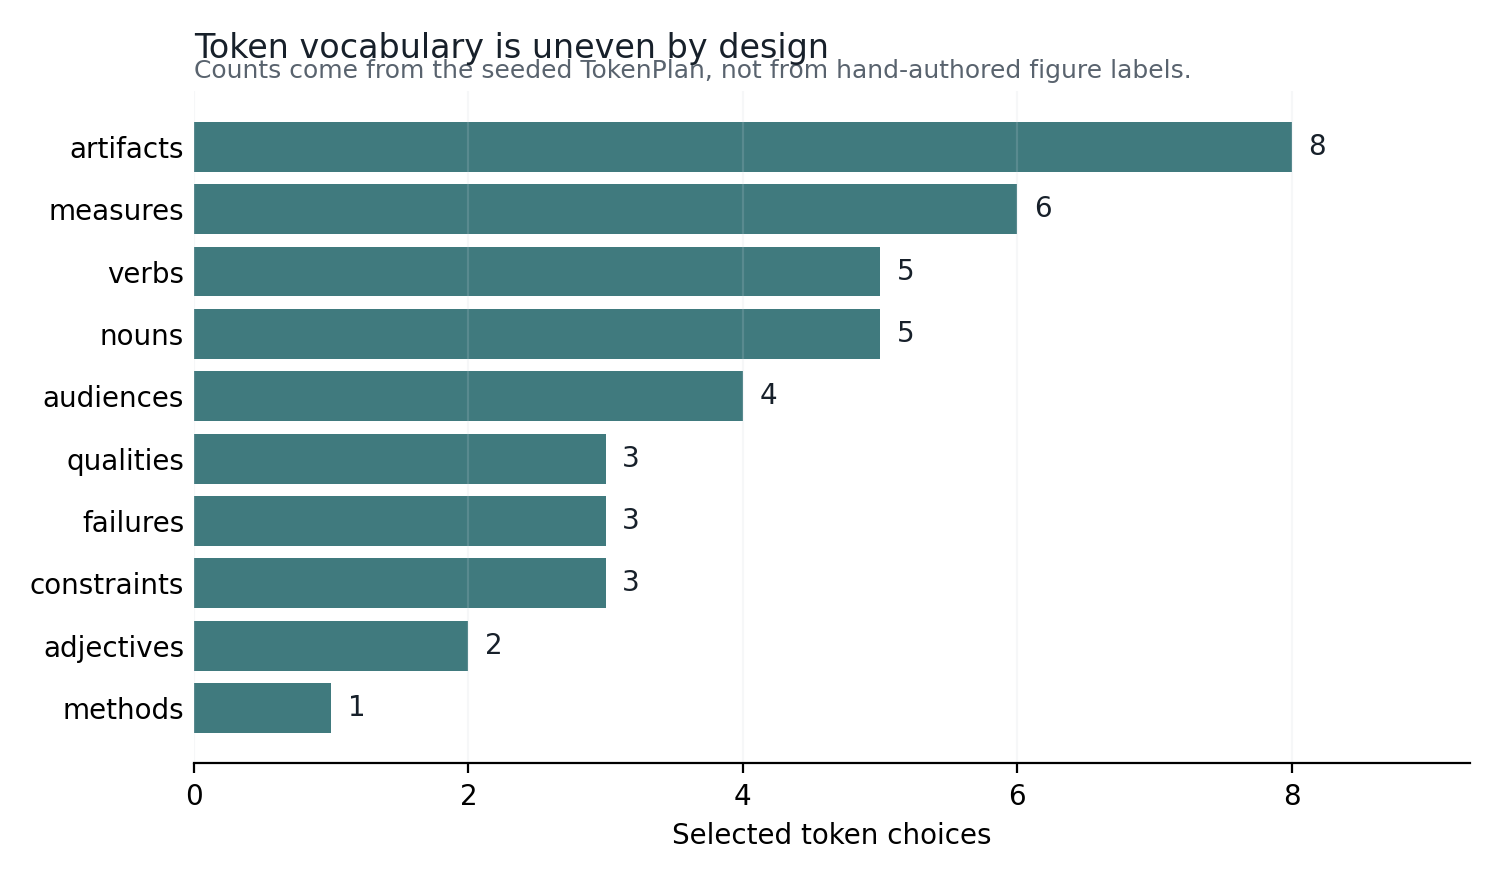
\includegraphics[keepaspectratio,alt={Token category density}]{../figures/token_density.png}}
\caption{Token category density}\label{fig:token-density}
\end{figure}

\begin{figure}
\centering
\pandocbounded{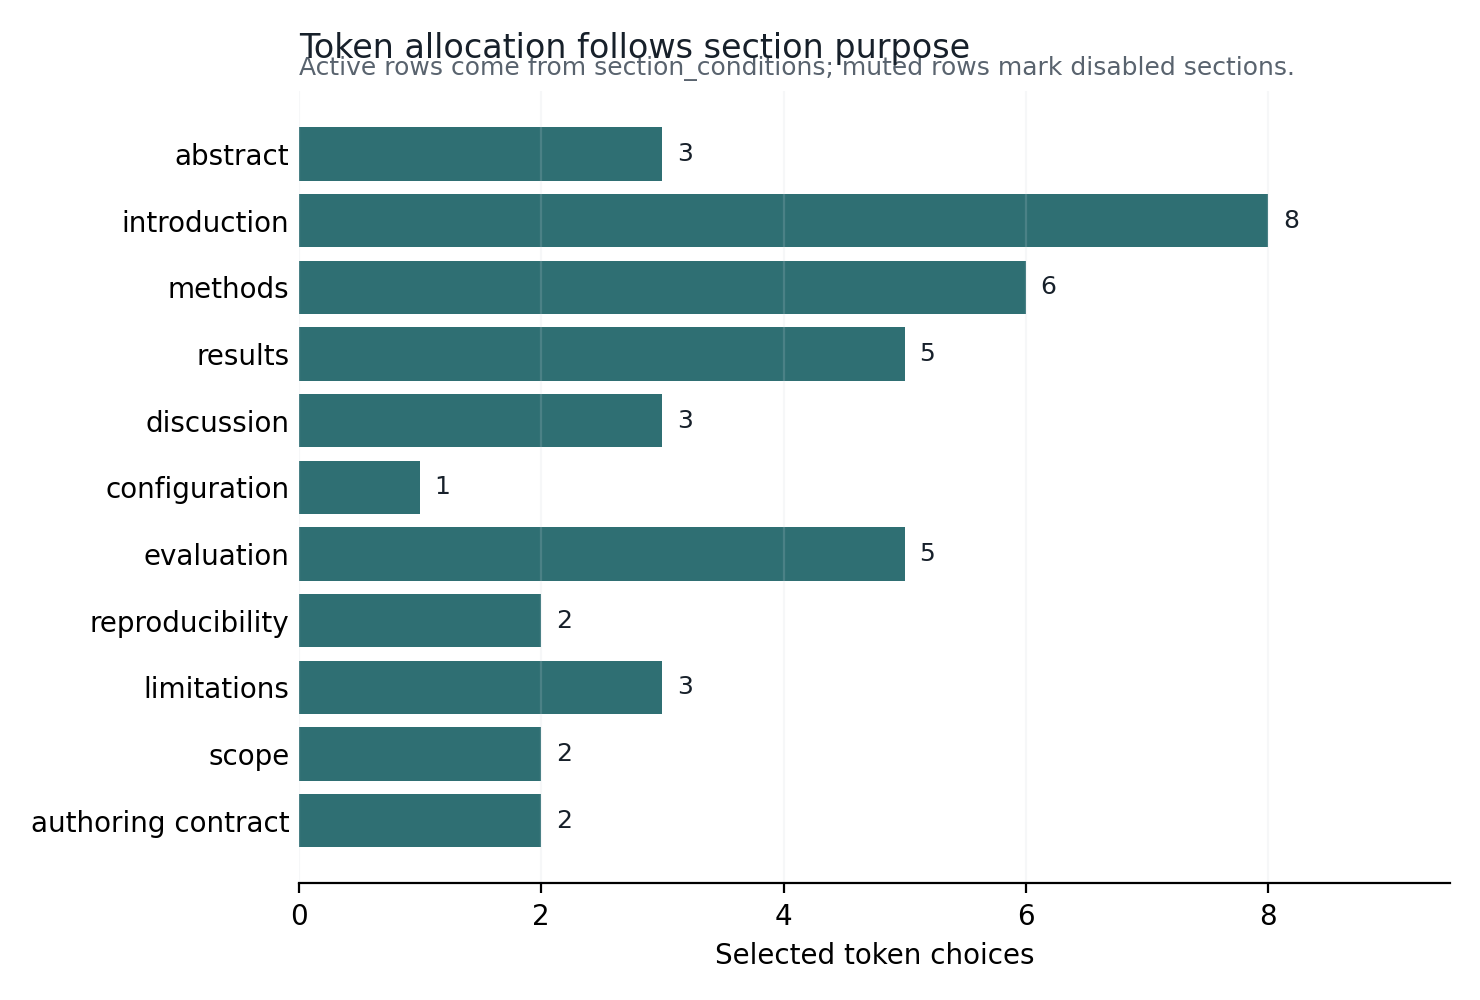
\includegraphics[keepaspectratio,alt={Section token allocation}]{../figures/section_token_allocation.png}}
\caption{Section token allocation}\label{fig:section-token-allocation}
\end{figure}

\begin{figure}
\centering
\pandocbounded{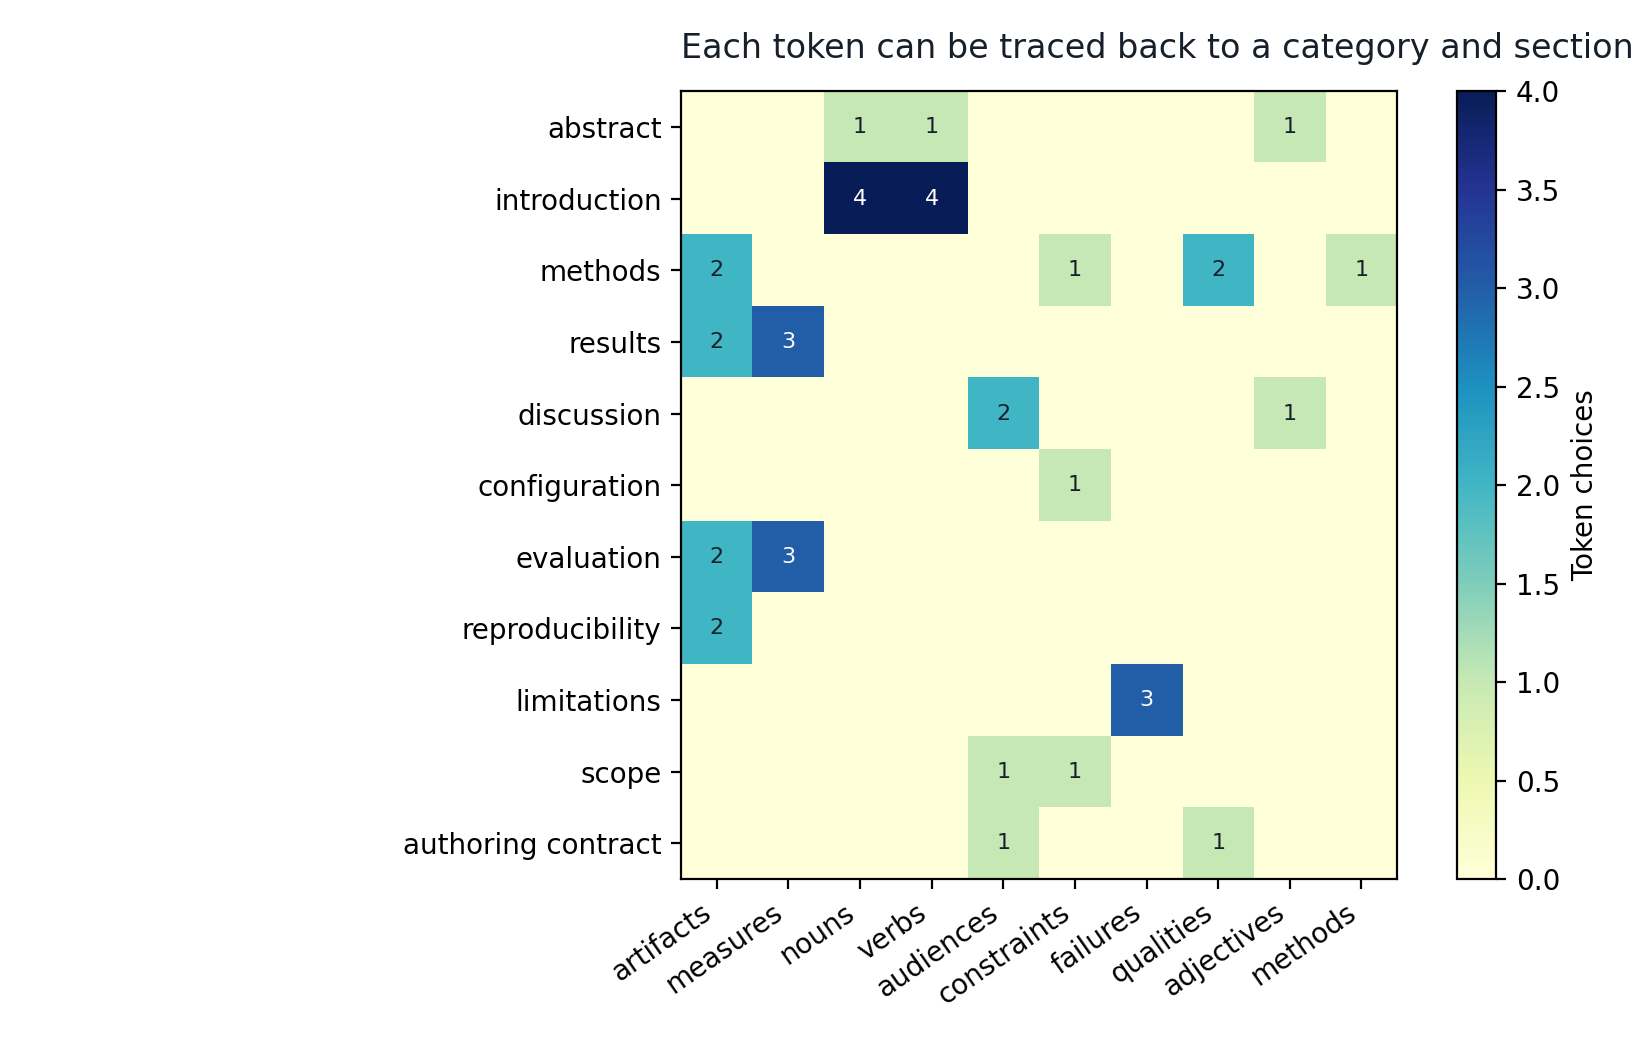
\includegraphics[keepaspectratio,alt={Provenance trace map}]{../figures/provenance_trace_map.png}}
\caption{Provenance trace map}\label{fig:provenance-trace-map}
\end{figure}

\subsection{Token Inventory}\label{token-inventory}

{\def\LTcaptype{none} % do not increment counter
\begin{longtable}[]{@{}
  >{\raggedright\arraybackslash}p{(\linewidth - 8\tabcolsep) * \real{0.2000}}
  >{\raggedright\arraybackslash}p{(\linewidth - 8\tabcolsep) * \real{0.2000}}
  >{\raggedright\arraybackslash}p{(\linewidth - 8\tabcolsep) * \real{0.2000}}
  >{\raggedright\arraybackslash}p{(\linewidth - 8\tabcolsep) * \real{0.2000}}
  >{\raggedright\arraybackslash}p{(\linewidth - 8\tabcolsep) * \real{0.2000}}@{}}
\toprule\noalign{}
\begin{minipage}[b]{\linewidth}\raggedright
Variable
\end{minipage} & \begin{minipage}[b]{\linewidth}\raggedright
Category
\end{minipage} & \begin{minipage}[b]{\linewidth}\raggedright
Value
\end{minipage} & \begin{minipage}[b]{\linewidth}\raggedright
Section
\end{minipage} & \begin{minipage}[b]{\linewidth}\raggedright
Source
\end{minipage} \\
\midrule\noalign{}
\endhead
\bottomrule\noalign{}
\endlastfoot
\texttt{STUDY\_ADJECTIVE} & adjectives & reviewable & abstract &
\texttt{manuscript/config.yaml\#madlib.lexicon.adjectives{[}5{]}} \\
\texttt{STUDY\_NOUN} & nouns & pipeline & abstract &
\texttt{manuscript/config.yaml\#madlib.lexicon.nouns{[}4{]}} \\
\texttt{STUDY\_VERB} & verbs & hydrate & abstract &
\texttt{manuscript/config.yaml\#madlib.lexicon.verbs{[}1{]}} \\
\texttt{INTRO\_NOUNS\_1} & nouns & protocol & introduction &
\texttt{manuscript/config.yaml\#madlib.lexicon.nouns{[}5{]}} \\
\texttt{INTRO\_NOUNS\_2} & nouns & section & introduction &
\texttt{manuscript/config.yaml\#madlib.lexicon.nouns{[}3{]}} \\
\texttt{INTRO\_NOUNS\_3} & nouns & lexicon & introduction &
\texttt{manuscript/config.yaml\#madlib.lexicon.nouns{[}2{]}} \\
\texttt{INTRO\_NOUNS\_4} & nouns & artifact & introduction &
\texttt{manuscript/config.yaml\#madlib.lexicon.nouns{[}6{]}} \\
\texttt{INTRO\_VERBS\_1} & verbs & condition & introduction &
\texttt{manuscript/config.yaml\#madlib.lexicon.verbs{[}3{]}} \\
\texttt{INTRO\_VERBS\_2} & verbs & bind & introduction &
\texttt{manuscript/config.yaml\#madlib.lexicon.verbs{[}6{]}} \\
\texttt{INTRO\_VERBS\_3} & verbs & bind & introduction &
\texttt{manuscript/config.yaml\#madlib.lexicon.verbs{[}6{]}} \\
\texttt{INTRO\_VERBS\_4} & verbs & compose & introduction &
\texttt{manuscript/config.yaml\#madlib.lexicon.verbs{[}0{]}} \\
\texttt{METHOD\_NAME} & methods & conditional section hydration &
methods &
\texttt{manuscript/config.yaml\#madlib.lexicon.methods{[}3{]}} \\
\breaktt{METHOD\_CONSTRAINT} & constraints & publication claims stay
local until release & methods &
\texttt{manuscript/config.yaml\#madlib.lexicon.constraints{[}3{]}} \\
\breaktt{METHOD\_ARTIFACT\_1} & artifacts & token-injection flow &
methods &
\texttt{manuscript/config.yaml\#madlib.lexicon.artifacts{[}6{]}} \\
\breaktt{METHOD\_ARTIFACT\_2} & artifacts & quality-gate matrix & methods
& \texttt{manuscript/config.yaml\#madlib.lexicon.artifacts{[}9{]}} \\
\breaktt{METHOD\_QUALITY\_1} & qualities & claim humility & methods &
\texttt{manuscript/config.yaml\#madlib.lexicon.qualities{[}4{]}} \\
\breaktt{METHOD\_QUALITY\_2} & qualities & render readiness & methods &
\texttt{manuscript/config.yaml\#madlib.lexicon.qualities{[}3{]}} \\
\breaktt{RESULT\_MEASURE\_1} & measures & provenance coverage & results &
\texttt{manuscript/config.yaml\#madlib.lexicon.measures{[}3{]}} \\
\breaktt{RESULT\_MEASURE\_2} & measures & evidence registry cleanliness &
results &
\texttt{manuscript/config.yaml\#madlib.lexicon.measures{[}6{]}} \\
\breaktt{RESULT\_MEASURE\_3} & measures & category density & results &
\texttt{manuscript/config.yaml\#madlib.lexicon.measures{[}2{]}} \\
\breaktt{RESULT\_ARTIFACT\_1} & artifacts & configured-field figures &
results &
\texttt{manuscript/config.yaml\#madlib.lexicon.artifacts{[}10{]}} \\
\breaktt{RESULT\_ARTIFACT\_2} & artifacts & token inventory & results &
\texttt{manuscript/config.yaml\#madlib.lexicon.artifacts{[}0{]}} \\
\breaktt{DISCUSSION\_ADJECTIVE} & adjectives & auditable & discussion &
\texttt{manuscript/config.yaml\#madlib.lexicon.adjectives{[}0{]}} \\
\breaktt{DISCUSSION\_AUDIENCE\_1} & audiences & pipeline maintainers &
discussion &
\texttt{manuscript/config.yaml\#madlib.lexicon.audiences{[}2{]}} \\
\breaktt{DISCUSSION\_AUDIENCE\_2} & audiences & research educators &
discussion &
\texttt{manuscript/config.yaml\#madlib.lexicon.audiences{[}3{]}} \\
\breaktt{CONFIG\_CONSTRAINT} & constraints & disabled sections retain
explicit traceability & configuration &
\texttt{manuscript/config.yaml\#madlib.lexicon.constraints{[}2{]}} \\
\breaktt{EVALUATION\_MEASURE\_1} & measures & copied output readiness &
evaluation &
\texttt{manuscript/config.yaml\#madlib.lexicon.measures{[}7{]}} \\
\breaktt{EVALUATION\_MEASURE\_2} & measures & figure registry
completeness & evaluation &
\texttt{manuscript/config.yaml\#madlib.lexicon.measures{[}5{]}} \\
\breaktt{EVALUATION\_MEASURE\_3} & measures & category density &
evaluation &
\texttt{manuscript/config.yaml\#madlib.lexicon.measures{[}2{]}} \\
\breaktt{EVALUATION\_ARTIFACT\_1} & artifacts & manuscript variable map &
evaluation &
\texttt{manuscript/config.yaml\#madlib.lexicon.artifacts{[}3{]}} \\
\breaktt{EVALUATION\_ARTIFACT\_2} & artifacts & provenance trace map &
evaluation &
\texttt{manuscript/config.yaml\#madlib.lexicon.artifacts{[}8{]}} \\
\breaktt{REPRODUCIBILITY\_ARTIFACT\_1} & artifacts & section plan &
reproducibility &
\texttt{manuscript/config.yaml\#madlib.lexicon.artifacts{[}1{]}} \\
\breaktt{REPRODUCIBILITY\_ARTIFACT\_2} & artifacts & manuscript variable
map & reproducibility &
\texttt{manuscript/config.yaml\#madlib.lexicon.artifacts{[}3{]}} \\
\breaktt{LIMITATION\_FAILURE\_1} & failures & domain misuse & limitations
& \texttt{manuscript/config.yaml\#madlib.lexicon.failures{[}4{]}} \\
\breaktt{LIMITATION\_FAILURE\_2} & failures & overclaimed generated prose
& limitations &
\texttt{manuscript/config.yaml\#madlib.lexicon.failures{[}1{]}} \\
\breaktt{LIMITATION\_FAILURE\_3} & failures & figure provenance gap &
limitations &
\texttt{manuscript/config.yaml\#madlib.lexicon.failures{[}3{]}} \\
\breaktt{SCOPE\_CONSTRAINT} & constraints & all lexicon entries live in
config & scope &
\texttt{manuscript/config.yaml\#madlib.lexicon.constraints{[}1{]}} \\
\texttt{SCOPE\_AUDIENCE} & audiences & pipeline maintainers & scope &
\texttt{manuscript/config.yaml\#madlib.lexicon.audiences{[}2{]}} \\
\breaktt{AUTHORING\_AUDIENCE} & audiences & manuscript reviewers &
authoring\_contract &
\texttt{manuscript/config.yaml\#madlib.lexicon.audiences{[}1{]}} \\
\breaktt{AUTHORING\_QUALITY} & qualities & render readiness &
authoring\_contract &
\texttt{manuscript/config.yaml\#madlib.lexicon.qualities{[}3{]}} \\
\end{longtable}
}

\subsection{Provenance Matrix}\label{provenance-matrix}

{\def\LTcaptype{none} % do not increment counter
\begin{longtable}[]{@{}
  >{\raggedright\arraybackslash}p{(\linewidth - 4\tabcolsep) * \real{0.3000}}
  >{\raggedleft\arraybackslash}p{(\linewidth - 4\tabcolsep) * \real{0.4000}}
  >{\raggedright\arraybackslash}p{(\linewidth - 4\tabcolsep) * \real{0.3000}}@{}}
\toprule\noalign{}
\begin{minipage}[b]{\linewidth}\raggedright
Section
\end{minipage} & \begin{minipage}[b]{\linewidth}\raggedleft
Token variables
\end{minipage} & \begin{minipage}[b]{\linewidth}\raggedright
Source categories
\end{minipage} \\
\midrule\noalign{}
\endhead
\bottomrule\noalign{}
\endlastfoot
Abstract & \texttt{STUDY\_ADJECTIVE}, \texttt{STUDY\_NOUN},
\texttt{STUDY\_VERB} & adjectives, nouns, verbs \\
Introduction: Lexicon as Data and Manuscript as Build Artifact &
\texttt{INTRO\_NOUNS\_1}, \texttt{INTRO\_NOUNS\_2},
\texttt{INTRO\_NOUNS\_3}, \texttt{INTRO\_NOUNS\_4},
\texttt{INTRO\_VERBS\_1}, \texttt{INTRO\_VERBS\_2},
\texttt{INTRO\_VERBS\_3}, \texttt{INTRO\_VERBS\_4} & nouns, verbs \\
Methods: Source-Owned Token Injection and Conditional IMRAD Assembly &
\texttt{METHOD\_NAME}, \breaktt{METHOD\_CONSTRAINT},
\breaktt{METHOD\_ARTIFACT\_1}, \breaktt{METHOD\_ARTIFACT\_2},
\breaktt{METHOD\_QUALITY\_1}, \breaktt{METHOD\_QUALITY\_2} & artifacts,
constraints, methods, qualities \\
Results: Provenance, Density, and Resolved Manuscript Surface &
\breaktt{RESULT\_MEASURE\_1}, \breaktt{RESULT\_MEASURE\_2},
\breaktt{RESULT\_MEASURE\_3}, \breaktt{RESULT\_ARTIFACT\_1},
\breaktt{RESULT\_ARTIFACT\_2} & artifacts, measures \\
Discussion: Accountability Boundaries for Generated Prose &
\breaktt{DISCUSSION\_ADJECTIVE}, \breaktt{DISCUSSION\_AUDIENCE\_1},
\breaktt{DISCUSSION\_AUDIENCE\_2} & adjectives, audiences \\
Configuration: Schema-Controlled Lexicon, Slots, and Narrative Moves &
\breaktt{CONFIG\_CONSTRAINT} & constraints \\
Evaluation: Gate Criteria, QA Probes, and Failure Discovery &
\breaktt{EVALUATION\_MEASURE\_1}, \breaktt{EVALUATION\_MEASURE\_2},
\breaktt{EVALUATION\_MEASURE\_3}, \breaktt{EVALUATION\_ARTIFACT\_1},
\breaktt{EVALUATION\_ARTIFACT\_2} & artifacts, measures \\
Reproducibility: Seeded Regeneration and Artifact Trace &
\breaktt{REPRODUCIBILITY\_ARTIFACT\_1},
\breaktt{REPRODUCIBILITY\_ARTIFACT\_2} & artifacts \\
Limitations: Non-Claims, Misuse Modes, and Human Review &
\breaktt{LIMITATION\_FAILURE\_1}, \breaktt{LIMITATION\_FAILURE\_2},
\breaktt{LIMITATION\_FAILURE\_3} & failures \\
Scope: Related Generators and Responsible Forking &
\breaktt{SCOPE\_CONSTRAINT}, \texttt{SCOPE\_AUDIENCE} & audiences,
constraints \\
Authoring Contract: Human Review and Forking Obligations &
\breaktt{AUTHORING\_AUDIENCE}, \breaktt{AUTHORING\_QUALITY} & audiences,
qualities \\
\end{longtable}
}

\newpage

\section{Discussion: Accountability Boundaries for Generated
Prose}\label{discussion-accountability-boundaries-for-generated-prose}

The reviewable result is intentionally modest. The exemplar does not
claim that random lexical replacement creates scholarship, discovers
facts, or substitutes for authorship. It shows that a conditional text
generator can be made accountable to configuration, tests, and
render-time validation.

The configured discussion moves are bound the scholarly claim, describe
useful adaptation cases, name misuse modes, and preserve human
authorship responsibility. Useful adaptations include templated
empirical reports, structured review memos, classroom exercises, and
manuscript sections that need to toggle across protocols. Risky
adaptations include hiding weak claims behind fluent generated phrasing
or allowing a token category to imply evidence that the project never
produced.

The pattern scales only when authors preserve the same ownership
boundary. Lexicons should be small enough to review, categories should
be named for their manuscript function, and section switches should
state what has been removed. When richer language is needed, the next
layer should add domain-specific validators rather than relaxing
provenance.

\newpage

\section{Configuration: Schema-Controlled Lexicon, Slots, and Narrative
Moves}\label{configuration-schema-controlled-lexicon-slots-and-narrative-moves}

The active composition depth is \texttt{deep}. The lexicon exposes 10
category list(s), and the slot declaration expands to 40 concrete token
choice(s). Section switches are evaluated before composition so disabled
sections cannot silently borrow enabled-section claims.

Configuration owns more than vocabulary. It also owns section titles,
narrative moves, method protocol rows, contribution claims, and audit
rules. That makes the manuscript shape visible in one YAML file while
preserving the rule that source code, not hand-edited output, performs
the composition.

The tables in this section expose the declared surface that controls
rendering. They are useful during review because a title change, slot
expansion, or disabled section appears as a small config diff and a
regenerated artifact diff rather than as scattered prose edits.

The configured-field inventory separates 125 explicit YAML path(s) from
11 loader-defaulted path(s). That distinction matters for forks: a field
that appears in the rendered manuscript may be intentionally authored in
\texttt{config.yaml}, or it may be a documented default inherited from
the template.

\begin{figure}
\centering
\pandocbounded{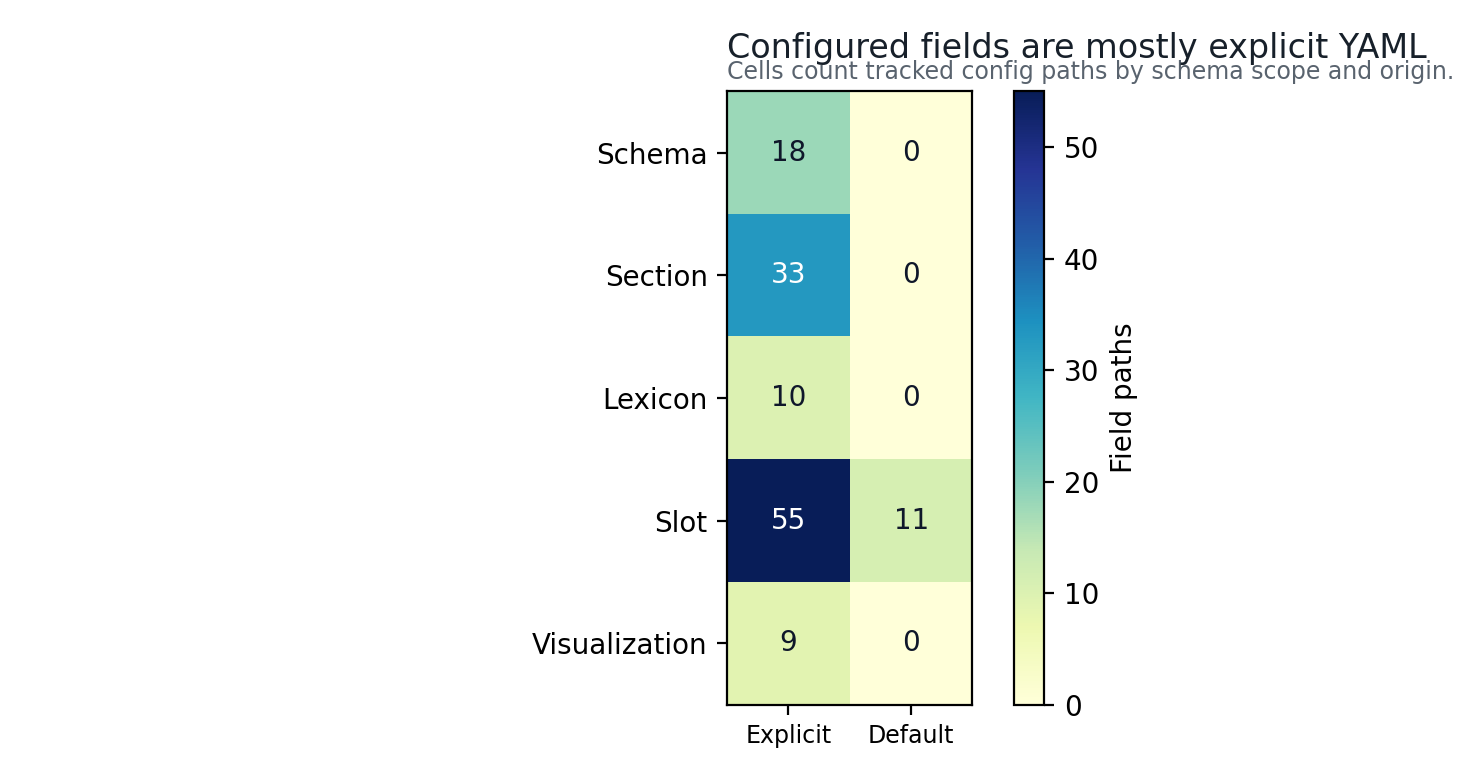
\includegraphics[keepaspectratio,alt={Configured field origin matrix}]{../figures/configured_field_matrix.png}}
\caption{Configured field origin
matrix}\label{fig:configured-field-matrix}
\end{figure}

\begin{figure}
\centering
\pandocbounded{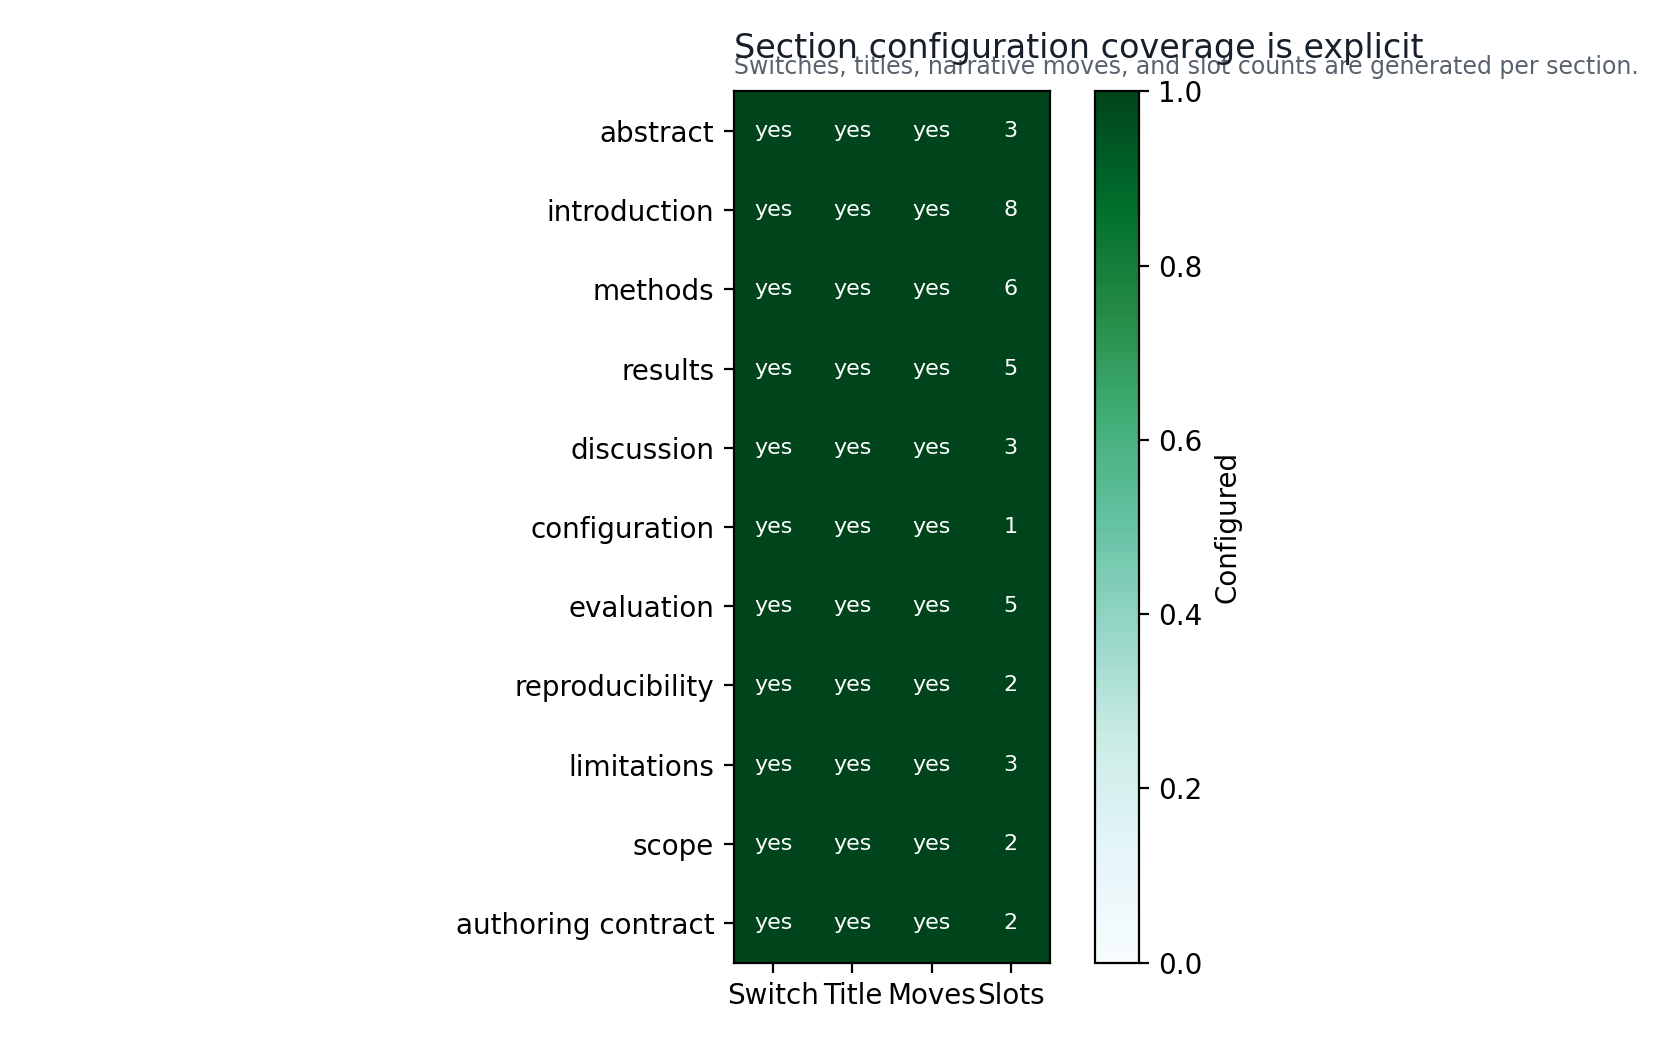
\includegraphics[keepaspectratio,alt={Section configuration heatmap}]{../figures/section_configuration_heatmap.png}}
\caption{Section configuration
heatmap}\label{fig:section-configuration-heatmap}
\end{figure}

\begin{figure}
\centering
\pandocbounded{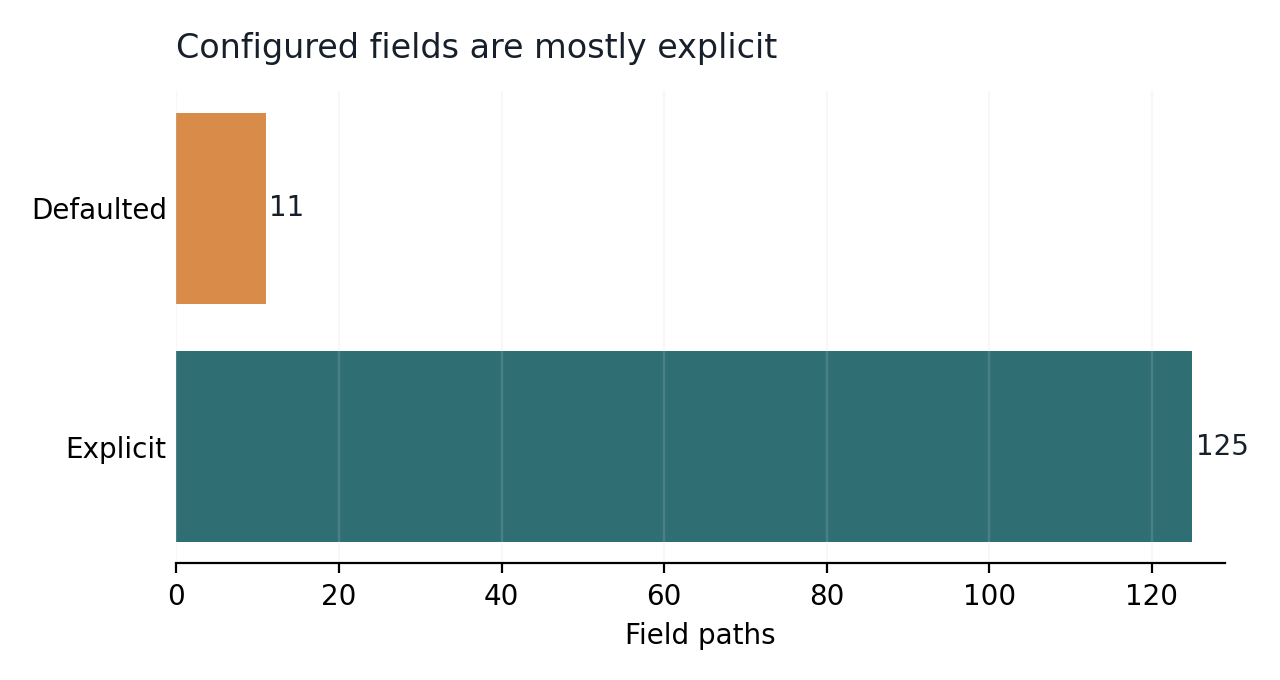
\includegraphics[keepaspectratio,alt={Field origin summary}]{../figures/field_origin_summary.png}}
\caption{Field origin summary}\label{fig:field-origin-summary}
\end{figure}

\subsection{Declared Section Titles}\label{declared-section-titles}

{\def\LTcaptype{none} % do not increment counter
\begin{longtable}[]{@{}
  >{\raggedright\arraybackslash}p{(\linewidth - 4\tabcolsep) * \real{0.3000}}
  >{\raggedright\arraybackslash}p{(\linewidth - 4\tabcolsep) * \real{0.3000}}
  >{\raggedleft\arraybackslash}p{(\linewidth - 4\tabcolsep) * \real{0.4000}}@{}}
\toprule\noalign{}
\begin{minipage}[b]{\linewidth}\raggedright
Section key
\end{minipage} & \begin{minipage}[b]{\linewidth}\raggedright
Rendered title
\end{minipage} & \begin{minipage}[b]{\linewidth}\raggedleft
Enabled
\end{minipage} \\
\midrule\noalign{}
\endhead
\bottomrule\noalign{}
\endlastfoot
\texttt{abstract} & Abstract & True \\
\texttt{introduction} & Introduction: Lexicon as Data and Manuscript as
Build Artifact & True \\
\texttt{methods} & Methods: Source-Owned Token Injection and Conditional
IMRAD Assembly & True \\
\texttt{results} & Results: Provenance, Density, and Resolved Manuscript
Surface & True \\
\texttt{discussion} & Discussion: Accountability Boundaries for
Generated Prose & True \\
\texttt{configuration} & Configuration: Schema-Controlled Lexicon,
Slots, and Narrative Moves & True \\
\texttt{evaluation} & Evaluation: Gate Criteria, QA Probes, and Failure
Discovery & True \\
\texttt{reproducibility} & Reproducibility: Seeded Regeneration and
Artifact Trace & True \\
\texttt{limitations} & Limitations: Non-Claims, Misuse Modes, and Human
Review & True \\
\texttt{scope} & Scope: Related Generators and Responsible Forking &
True \\
\breaktt{authoring\_contract} & Authoring Contract: Human Review and
Forking Obligations & True \\
\end{longtable}
}

\subsection{Configuration Counts}\label{configuration-counts}

\begin{itemize}
\tightlist
\item
  Seed: \texttt{431}
\item
  Composition depth: \texttt{deep}
\item
  Lexicon categories: \texttt{10}
\item
  Slot rules: \texttt{22}
\item
  Token choices: \texttt{40}
\item
  Enabled sections: \texttt{11}
\item
  Method steps: \texttt{18}
\item
  Design principles: \texttt{13}
\item
  Pipeline phases: \texttt{17}
\item
  Quality probes: \texttt{14}
\item
  Authoring obligations: \texttt{8}
\item
  Explicit configured paths: \texttt{125}
\item
  Defaulted configured paths: \texttt{11}
\item
  Enabled visualization flags: \texttt{7}
\item
  Section-level configured paths: \texttt{33}
\item
  Lexicon-level configured paths: \texttt{10}
\item
  Slot-level configured paths: \texttt{66}
\item
  Narrative moves: \texttt{52}
\item
  Audit rules: \texttt{12}
\item
  Contribution claims: \texttt{9}
\end{itemize}

\subsection{Configured Field Summary}\label{configured-field-summary}

{\def\LTcaptype{none} % do not increment counter
\begin{longtable}[]{@{}lr@{}}
\toprule\noalign{}
Measure & Count \\
\midrule\noalign{}
\endhead
\bottomrule\noalign{}
\endlastfoot
Total tracked field paths & 136 \\
Explicit YAML paths & 125 \\
Loader-defaulted paths & 11 \\
Enabled visualization flags & 7 \\
Section-level paths & 33 \\
Lexicon-level paths & 10 \\
Slot-level paths & 66 \\
Visualization-control paths & 9 \\
Top-level schema paths & 18 \\
\end{longtable}
}

\subsection{Configured Field
Inventory}\label{configured-field-inventory}

{\def\LTcaptype{none} % do not increment counter
\begin{longtable}[]{@{}
  >{\raggedright\arraybackslash}p{(\linewidth - 6\tabcolsep) * \real{0.2500}}
  >{\raggedright\arraybackslash}p{(\linewidth - 6\tabcolsep) * \real{0.2500}}
  >{\raggedright\arraybackslash}p{(\linewidth - 6\tabcolsep) * \real{0.2500}}
  >{\raggedright\arraybackslash}p{(\linewidth - 6\tabcolsep) * \real{0.2500}}@{}}
\toprule\noalign{}
\begin{minipage}[b]{\linewidth}\raggedright
Path
\end{minipage} & \begin{minipage}[b]{\linewidth}\raggedright
Origin
\end{minipage} & \begin{minipage}[b]{\linewidth}\raggedright
Scope
\end{minipage} & \begin{minipage}[b]{\linewidth}\raggedright
Summary
\end{minipage} \\
\midrule\noalign{}
\endhead
\bottomrule\noalign{}
\endlastfoot
\texttt{madlib} & explicit & schema & configured field \\
\breaktt{madlib.audit\_rules} & explicit & schema & 12 entries \\
\breaktt{madlib.authoring\_obligations} & explicit & schema & 8
entries \\
\breaktt{madlib.composition\_depth} & explicit & schema & deep \\
\breaktt{madlib.contribution\_claims} & explicit & schema & 9 entries \\
\breaktt{madlib.design\_principles} & explicit & schema & 13 entries \\
\breaktt{madlib.evaluation\_criteria} & explicit & schema & 7 entries \\
\breaktt{madlib.failure\_modes} & explicit & schema & 13 entries \\
\breaktt{madlib.hypothesis} & explicit & schema & Deterministic lexical
injection can generate a complete conditional IMRAD manuscript while
preserving token provenance, section intent, and audit-ready method
evidence. \\
\texttt{madlib.lexicon} & explicit & schema & 10 categories \\
\breaktt{madlib.lexicon.adjectives} & explicit & lexicon & 7 tokens \\
\breaktt{madlib.lexicon.artifacts} & explicit & lexicon & 12 tokens \\
\breaktt{madlib.lexicon.audiences} & explicit & lexicon & 4 tokens \\
\breaktt{madlib.lexicon.constraints} & explicit & lexicon & 5 tokens \\
\breaktt{madlib.lexicon.failures} & explicit & lexicon & 5 tokens \\
\breaktt{madlib.lexicon.measures} & explicit & lexicon & 8 tokens \\
\breaktt{madlib.lexicon.methods} & explicit & lexicon & 5 tokens \\
\breaktt{madlib.lexicon.nouns} & explicit & lexicon & 7 tokens \\
\breaktt{madlib.lexicon.qualities} & explicit & lexicon & 5 tokens \\
\breaktt{madlib.lexicon.verbs} & explicit & lexicon & 7 tokens \\
\breaktt{madlib.method\_protocol} & explicit & schema & 18 entries \\
\breaktt{madlib.narrative\_moves} & explicit & schema & configured
field \\
\breaktt{madlib.narrative\_moves.abstract} & explicit & section & 3
moves \\
\breaktt{madlib.narrative\_moves.authoring\_contract} & explicit &
section & 5 moves \\
\breaktt{madlib.narrative\_moves.configuration} & explicit & section & 3
moves \\
\breaktt{madlib.narrative\_moves.discussion} & explicit & section & 4
moves \\
\breaktt{madlib.narrative\_moves.evaluation} & explicit & section & 4
moves \\
\breaktt{madlib.narrative\_moves.introduction} & explicit & section & 4
moves \\
\breaktt{madlib.narrative\_moves.limitations} & explicit & section & 4
moves \\
\breaktt{madlib.narrative\_moves.methods} & explicit & section & 13
moves \\
\breaktt{madlib.narrative\_moves.reproducibility} & explicit & section &
4 moves \\
\breaktt{madlib.narrative\_moves.results} & explicit & section & 4
moves \\
\breaktt{madlib.narrative\_moves.scope} & explicit & section & 4 moves \\
\breaktt{madlib.pipeline\_phases} & explicit & schema & 17 entries \\
\breaktt{madlib.quality\_probes} & explicit & schema & 14 entries \\
\breaktt{madlib.section\_conditions} & explicit & schema & configured
field \\
\breaktt{madlib.section\_conditions.abstract} & explicit & section &
enabled \\
\breaktt{madlib.section\_conditions.authoring\_contract} & explicit &
section & enabled \\
\breaktt{madlib.section\_conditions.configuration} & explicit & section &
enabled \\
\breaktt{madlib.section\_conditions.discussion} & explicit & section &
enabled \\
\breaktt{madlib.section\_conditions.evaluation} & explicit & section &
enabled \\
\breaktt{madlib.section\_conditions.introduction} & explicit & section &
enabled \\
\breaktt{madlib.section\_conditions.limitations} & explicit & section &
enabled \\
\breaktt{madlib.section\_conditions.methods} & explicit & section &
enabled \\
\breaktt{madlib.section\_conditions.reproducibility} & explicit & section
& enabled \\
\breaktt{madlib.section\_conditions.results} & explicit & section &
enabled \\
\breaktt{madlib.section\_conditions.scope} & explicit & section &
enabled \\
\breaktt{madlib.section\_titles} & explicit & schema & configured
field \\
\breaktt{madlib.section\_titles.abstract} & explicit & section &
Abstract \\
\breaktt{madlib.section\_titles.authoring\_contract} & explicit & section
& Authoring Contract: Human Review and Forking Obligations \\
\breaktt{madlib.section\_titles.configuration} & explicit & section &
Configuration: Schema-Controlled Lexicon, Slots, and Narrative Moves \\
\breaktt{madlib.section\_titles.discussion} & explicit & section &
Discussion: Accountability Boundaries for Generated Prose \\
\breaktt{madlib.section\_titles.evaluation} & explicit & section &
Evaluation: Gate Criteria, QA Probes, and Failure Discovery \\
\breaktt{madlib.section\_titles.introduction} & explicit & section &
Introduction: Lexicon as Data and Manuscript as Build Artifact \\
\breaktt{madlib.section\_titles.limitations} & explicit & section &
Limitations: Non-Claims, Misuse Modes, and Human Review \\
\breaktt{madlib.section\_titles.methods} & explicit & section & Methods:
Source-Owned Token Injection and Conditional IMRAD Assembly \\
\breaktt{madlib.section\_titles.reproducibility} & explicit & section &
Reproducibility: Seeded Regeneration and Artifact Trace \\
\breaktt{madlib.section\_titles.results} & explicit & section & Results:
Provenance, Density, and Resolved Manuscript Surface \\
\breaktt{madlib.section\_titles.scope} & explicit & section & Scope:
Related Generators and Responsible Forking \\
\texttt{madlib.seed} & explicit & schema & 431 \\
\texttt{madlib.slots} & explicit & schema & 22 slot rules, 40 token
choices \\
\breaktt{madlib.slots.authoring\_audience} & explicit & slot & audiences
-\textgreater{} authoring\_contract (1) \\
\breaktt{madlib.slots.authoring\_audience.count} & defaulted & slot &
1 \\
\breaktt{madlib.slots.authoring\_audience.section} & explicit & slot &
authoring\_contract \\
\breaktt{madlib.slots.authoring\_quality} & explicit & slot & qualities
-\textgreater{} authoring\_contract (1) \\
\breaktt{madlib.slots.authoring\_quality.count} & defaulted & slot & 1 \\
\breaktt{madlib.slots.authoring\_quality.section} & explicit & slot &
authoring\_contract \\
\breaktt{madlib.slots.config\_constraint} & explicit & slot & constraints
-\textgreater{} configuration (1) \\
\breaktt{madlib.slots.config\_constraint.count} & defaulted & slot & 1 \\
\breaktt{madlib.slots.config\_constraint.section} & explicit & slot &
configuration \\
\breaktt{madlib.slots.discussion\_adjective} & explicit & slot &
adjectives -\textgreater{} discussion (1) \\
\breaktt{madlib.slots.discussion\_adjective.count} & defaulted & slot &
1 \\
\breaktt{madlib.slots.discussion\_adjective.section} & explicit & slot &
discussion \\
\breaktt{madlib.slots.discussion\_audience} & explicit & slot & audiences
-\textgreater{} discussion (2) \\
\breaktt{madlib.slots.discussion\_audience.count} & explicit & slot &
2 \\
\breaktt{madlib.slots.discussion\_audience.section} & explicit & slot &
discussion \\
\breaktt{madlib.slots.evaluation\_artifact} & explicit & slot & artifacts
-\textgreater{} evaluation (2) \\
\breaktt{madlib.slots.evaluation\_artifact.count} & explicit & slot &
2 \\
\breaktt{madlib.slots.evaluation\_artifact.section} & explicit & slot &
evaluation \\
\breaktt{madlib.slots.evaluation\_measure} & explicit & slot & measures
-\textgreater{} evaluation (3) \\
\breaktt{madlib.slots.evaluation\_measure.count} & explicit & slot & 3 \\
\breaktt{madlib.slots.evaluation\_measure.section} & explicit & slot &
evaluation \\
\breaktt{madlib.slots.intro\_nouns} & explicit & slot & nouns
-\textgreater{} introduction (4) \\
\breaktt{madlib.slots.intro\_nouns.count} & explicit & slot & 4 \\
\breaktt{madlib.slots.intro\_nouns.section} & explicit & slot &
introduction \\
\breaktt{madlib.slots.intro\_verbs} & explicit & slot & verbs
-\textgreater{} introduction (4) \\
\breaktt{madlib.slots.intro\_verbs.count} & explicit & slot & 4 \\
\breaktt{madlib.slots.intro\_verbs.section} & explicit & slot &
introduction \\
\breaktt{madlib.slots.limitation\_failure} & explicit & slot & failures
-\textgreater{} limitations (3) \\
\breaktt{madlib.slots.limitation\_failure.count} & explicit & slot & 3 \\
\breaktt{madlib.slots.limitation\_failure.section} & explicit & slot &
limitations \\
\breaktt{madlib.slots.method\_artifact} & explicit & slot & artifacts
-\textgreater{} methods (2) \\
\breaktt{madlib.slots.method\_artifact.count} & explicit & slot & 2 \\
\breaktt{madlib.slots.method\_artifact.section} & explicit & slot &
methods \\
\breaktt{madlib.slots.method\_constraint} & explicit & slot & constraints
-\textgreater{} methods (1) \\
\breaktt{madlib.slots.method\_constraint.count} & defaulted & slot & 1 \\
\breaktt{madlib.slots.method\_constraint.section} & explicit & slot &
methods \\
\breaktt{madlib.slots.method\_name} & explicit & slot & methods
-\textgreater{} methods (1) \\
\breaktt{madlib.slots.method\_name.count} & defaulted & slot & 1 \\
\breaktt{madlib.slots.method\_name.section} & explicit & slot &
methods \\
\breaktt{madlib.slots.method\_quality} & explicit & slot & qualities
-\textgreater{} methods (2) \\
\breaktt{madlib.slots.method\_quality.count} & explicit & slot & 2 \\
\breaktt{madlib.slots.method\_quality.section} & explicit & slot &
methods \\
\breaktt{madlib.slots.reproducibility\_artifact} & explicit & slot &
artifacts -\textgreater{} reproducibility (2) \\
\breaktt{madlib.slots.reproducibility\_artifact.count} & explicit & slot
& 2 \\
\breaktt{madlib.slots.reproducibility\_artifact.section} & explicit &
slot & reproducibility \\
\breaktt{madlib.slots.result\_artifact} & explicit & slot & artifacts
-\textgreater{} results (2) \\
\breaktt{madlib.slots.result\_artifact.count} & explicit & slot & 2 \\
\breaktt{madlib.slots.result\_artifact.section} & explicit & slot &
results \\
\breaktt{madlib.slots.result\_measure} & explicit & slot & measures
-\textgreater{} results (3) \\
\breaktt{madlib.slots.result\_measure.count} & explicit & slot & 3 \\
\breaktt{madlib.slots.result\_measure.section} & explicit & slot &
results \\
\breaktt{madlib.slots.scope\_audience} & explicit & slot & audiences
-\textgreater{} scope (1) \\
\breaktt{madlib.slots.scope\_audience.count} & defaulted & slot & 1 \\
\breaktt{madlib.slots.scope\_audience.section} & explicit & slot &
scope \\
\breaktt{madlib.slots.scope\_constraint} & explicit & slot & constraints
-\textgreater{} scope (1) \\
\breaktt{madlib.slots.scope\_constraint.count} & defaulted & slot & 1 \\
\breaktt{madlib.slots.scope\_constraint.section} & explicit & slot &
scope \\
\breaktt{madlib.slots.study\_adjective} & explicit & slot & adjectives
-\textgreater{} abstract (1) \\
\breaktt{madlib.slots.study\_adjective.count} & defaulted & slot & 1 \\
\breaktt{madlib.slots.study\_adjective.section} & explicit & slot &
abstract \\
\breaktt{madlib.slots.study\_noun} & explicit & slot & nouns
-\textgreater{} abstract (1) \\
\breaktt{madlib.slots.study\_noun.count} & defaulted & slot & 1 \\
\breaktt{madlib.slots.study\_noun.section} & explicit & slot &
abstract \\
\breaktt{madlib.slots.study\_verb} & explicit & slot & verbs
-\textgreater{} abstract (1) \\
\breaktt{madlib.slots.study\_verb.count} & defaulted & slot & 1 \\
\breaktt{madlib.slots.study\_verb.section} & explicit & slot &
abstract \\
\breaktt{madlib.visualizations} & explicit & visualization & enabled \\
\breaktt{madlib.visualizations.configured\_field\_matrix} & explicit &
visualization & true \\
\breaktt{madlib.visualizations.enabled} & explicit & visualization &
true \\
\breaktt{madlib.visualizations.field\_origin\_summary} & explicit &
visualization & true \\
\breaktt{madlib.visualizations.provenance\_trace\_map} & explicit &
visualization & true \\
\breaktt{madlib.visualizations.quality\_gate\_matrix} & explicit &
visualization & true \\
\breaktt{madlib.visualizations.section\_configuration\_heatmap} &
explicit & visualization & true \\
\breaktt{madlib.visualizations.section\_token\_allocation} & explicit &
visualization & true \\
\breaktt{madlib.visualizations.token\_injection\_flow} & explicit &
visualization & true \\
\end{longtable}
}

\newpage

\section{Evaluation: Gate Criteria, QA Probes, and Failure
Discovery}\label{evaluation-gate-criteria-qa-probes-and-failure-discovery}

The evaluation section is configured to name readiness criteria, connect
criteria to artifacts, separate local checks from publication readiness,
and make failure probes visible. The local readiness surface is not a
human preference score; it is a set of deterministic checks that connect
generated manuscript claims to source files and pipeline gates.

The active criteria use analysis, copy, pytest, validation as gate
labels and inspect artifacts such as token-injection flow, quality-gate
matrix, configured-field figures. A passing run means the exemplar is
locally render-ready: placeholders resolve, token provenance is present,
figure references are registered, evidence scanning has not found
unsupported numbers, and project design overlays remain internally
consistent.

That readiness is deliberately narrower than publication readiness. A
local pass does not imply a standalone DOI, external release, reader
preference result, or empirical validation. It means the tracked project
tree can regenerate the committed artifact surface through its declared
pipeline.

The QA probes are Method row completeness, Field-origin visibility,
Placeholder survival, Provenance completeness, Section-switch
observability, Figure registry coverage, Method-figure alignment,
Evidence cleanliness, Fork readiness, Copied-output parity, Digest
invariant review, Claim-ledger alignment, Review packet completeness,
Fork migration sufficiency. They are phrased as questions so they can be
reused by reviewers and by forks of the exemplar: did the placeholder
disappear, did the provenance survive, did the figure registry cover
every reference, and did copied outputs preserve the same evidence
surface that validation inspected?

\begin{figure}
\centering
\pandocbounded{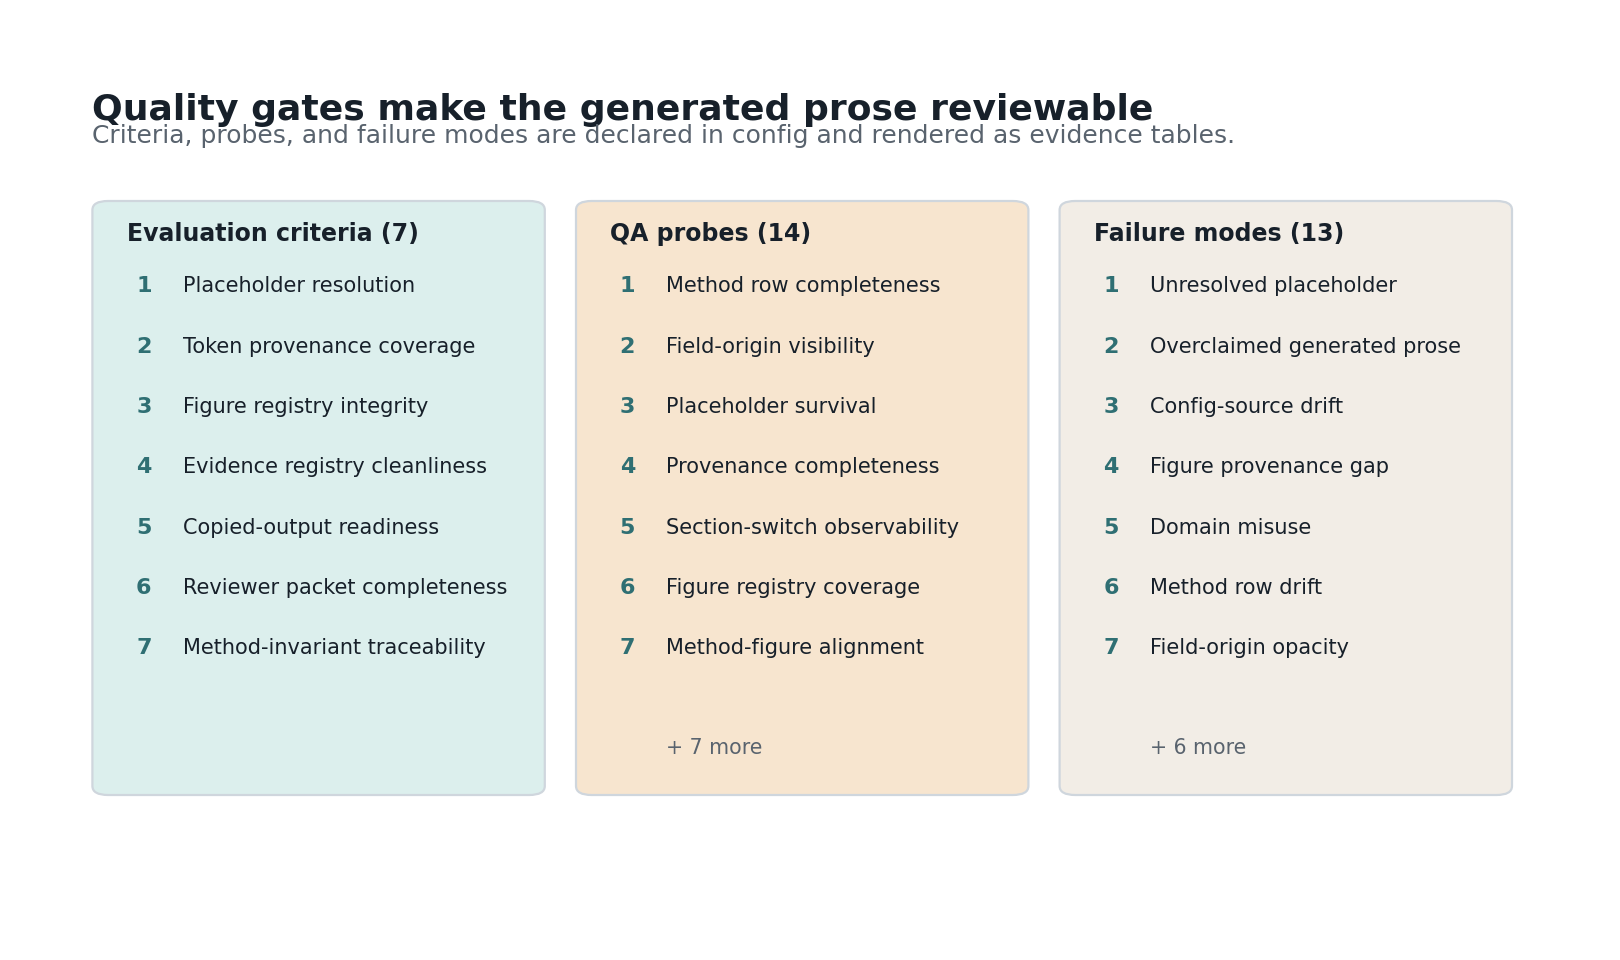
\includegraphics[keepaspectratio,alt={Quality gate matrix}]{../figures/quality_gate_matrix.png}}
\caption{Quality gate matrix}\label{fig:quality-gate-matrix}
\end{figure}

\subsection{Evaluation Criteria}\label{evaluation-criteria}

{\def\LTcaptype{none} % do not increment counter
\begin{longtable}[]{@{}
  >{\raggedright\arraybackslash}p{(\linewidth - 6\tabcolsep) * \real{0.2500}}
  >{\raggedright\arraybackslash}p{(\linewidth - 6\tabcolsep) * \real{0.2500}}
  >{\raggedright\arraybackslash}p{(\linewidth - 6\tabcolsep) * \real{0.2500}}
  >{\raggedright\arraybackslash}p{(\linewidth - 6\tabcolsep) * \real{0.2500}}@{}}
\toprule\noalign{}
\begin{minipage}[b]{\linewidth}\raggedright
Criterion
\end{minipage} & \begin{minipage}[b]{\linewidth}\raggedright
Target
\end{minipage} & \begin{minipage}[b]{\linewidth}\raggedright
Evidence
\end{minipage} & \begin{minipage}[b]{\linewidth}\raggedright
Gate
\end{minipage} \\
\midrule\noalign{}
\endhead
\bottomrule\noalign{}
\endlastfoot
Placeholder resolution & No unresolved uppercase manuscript placeholders
remain in output/manuscript or rendered web output. &
tests/test\_manuscript\_variables.py and rg unresolved-token scan. &
\texttt{pytest} \\
Token provenance coverage & Every selected token maps to category,
selected value, section, and config pointer. &
output/reports/injection\_trace.json and
output/data/token\_inventory.json. & \texttt{analysis} \\
Figure registry integrity & Every referenced figure label is present in
../figures/figure\_registry.json. & scripts/04\_validate\_output.py
figure registry check. & \texttt{validation} \\
Evidence registry cleanliness & Generated manuscript numbers and claims
pass the project evidence registry. &
output/reports/evidence\_registry.json. & \texttt{validation} \\
Copied-output readiness & PDF, HTML, slides, figures, data, and reports
copy into output/templates/template\_madlib. &
scripts/05\_copy\_outputs.py output statistics. & \texttt{copy} \\
Reviewer packet completeness & Hydrated Markdown, rendered PDF, web
output, slides, figures, data, reports, validation results, and copy
statistics are all present for review. & Stage 04 validation report and
Stage 05 output\_statistics.json. & \texttt{copy} \\
Method-invariant traceability & Token choices can be explained only by
seed, slot, category, ordinal, and ordered category inventory. &
tests/test\_tokens.py and generated Methods digest prose. &
\texttt{pytest} \\
\end{longtable}
}

\subsection{Quality Probes}\label{quality-probes}

{\def\LTcaptype{none} % do not increment counter
\begin{longtable}[]{@{}
  >{\raggedright\arraybackslash}p{(\linewidth - 6\tabcolsep) * \real{0.2500}}
  >{\raggedright\arraybackslash}p{(\linewidth - 6\tabcolsep) * \real{0.2500}}
  >{\raggedright\arraybackslash}p{(\linewidth - 6\tabcolsep) * \real{0.2500}}
  >{\raggedright\arraybackslash}p{(\linewidth - 6\tabcolsep) * \real{0.2500}}@{}}
\toprule\noalign{}
\begin{minipage}[b]{\linewidth}\raggedright
Probe
\end{minipage} & \begin{minipage}[b]{\linewidth}\raggedright
Question
\end{minipage} & \begin{minipage}[b]{\linewidth}\raggedright
Passing signal
\end{minipage} & \begin{minipage}[b]{\linewidth}\raggedright
Artifact
\end{minipage} \\
\midrule\noalign{}
\endhead
\bottomrule\noalign{}
\endlastfoot
Method row completeness & Does the protocol table cover schema intake,
token planning, composition, figures, validation, copy, and review
handoff? & method\_protocol includes rows for every major pipeline
responsibility. &
\breaktt{manuscript/config.yaml\ and\ output/data/section\_plan.json} \\
Field-origin visibility & Can a reviewer tell which visible fields were
authored and which were defaulted? & Configured-field inventory and
summary tables report explicit and defaulted paths. &
\breaktt{output/data/configured\_field\_inventory.json} \\
Placeholder survival & Did any source token survive hydration? & No
uppercase placeholders are found in generated manuscript or web files. &
\breaktt{output/manuscript\ and\ output/web} \\
Provenance completeness & Can every selected token be traced to a
category, section, value, and config key? & The injection trace and
token inventory contain one row for each generated token. &
\breaktt{output/reports/injection\_trace.json} \\
Section-switch observability & Does a disabled section resolve to a
visible explanation? & Disabled section bodies cite their controlling
section condition. & \breaktt{output/data/section\_plan.json} \\
Figure registry coverage & Does every manuscript figure reference have a
generated registry entry? & Figure registry validation passes. &
\breaktt{../figures/figure\_registry.json} \\
Method-figure alignment & Do method figures describe generated data
rather than decorative or unsupported claims? & Figure registry
captions, nonblank PNG tests, and manual visual QA align with artifact
data. & \texttt{output/figures} \\
Evidence cleanliness & Do generated claims stay within local evidence
boundaries? & Evidence registry validation passes without unsupported
claims. & \breaktt{output/reports/evidence\_registry.json} \\
Fork readiness & Does the authoring contract tell downstream forks what
to extend before adding domain claims? & Authoring obligations cite
config diffs, claim ledger updates, validators, and full reruns. &
\breaktt{output/manuscript/10\_authoring\_contract.md} \\
Copied-output parity & Did copied deliverables preserve the validated
project output surface? & Copy-stage statistics include PDF, HTML,
slides, figures, data, and reports. &
\breaktt{output/templates/template\_madlib} \\
Digest invariant review & Are the allowed token-selection inputs
documented and protected by tests? & Methods prose names the digest
inputs and token tests prove seed/category sensitivity. &
\breaktt{src/tokens.py\ and\ output/manuscript/02\_methodology.md} \\
Claim-ledger alignment & Do method and documentation claims point to
config, source, generated artifacts, or explicit non-claim boundaries? &
Claim-ledger rows cover expanded method protocol and fork-validator
boundaries. & \breaktt{data/claim\_ledger.yaml} \\
Review packet completeness & Can a reviewer inspect every output surface
needed to audit the method? & Copied outputs include manuscript, web,
slides, figures, data, reports, validation, and copy statistics. &
\breaktt{output/templates/template\_madlib\ and\ output/reports/output\_statistics.json} \\
Fork migration sufficiency & Does the documentation tell forks which
surfaces to change before adding domain claims? & README, STANDALONE,
manuscript README, and Authoring Contract list config, source, test,
validator, and claim-ledger obligations. &
\breaktt{README.md,\ STANDALONE.md,\ manuscript/README.md,\ and\ output/manuscript/10\_authoring\_contract.md} \\
\end{longtable}
}

\newpage

\section{Reproducibility: Seeded Regeneration and Artifact
Trace}\label{reproducibility-seeded-regeneration-and-artifact-trace}

Re-running generation with seed \texttt{431} and the same lexicon
produces the same token plan. The artifact set records
\breaktt{token\_inventory.json}, \breaktt{section\_plan.json},
\breaktt{injection\_trace.json}, \breaktt{manuscript\_variables.json},
\breaktt{figure\_registry.json}, and the
cover/results/configuration/evaluation figure set so the manuscript can
be audited without reading the PDF.

The protocol emits MadlibConfig, review scenario, explicit/default path
inventory, validated lexicon, digest input records, selection invariant
set, TokenPlan, enabled section set, section variables, Markdown
evidence tables, claim-aligned evidence surface, registered figure set,
output/data, output/reports, and output/figures, output/manuscript,
validated project output, review packet, copied publication-review
bundle, fork migration notes. Project tests cover deterministic token
choice, seed sensitivity, category-input sensitivity, malformed config
rejection, section disablement, artifact writing, and unresolved
manuscript-token detection. The shared output validator then checks
rendered PDFs, Markdown, figure registry, evidence registry, and design
overlays.

The copied root output is therefore a consequence of local source and
config. Generated files remain disposable; the durable contract is the
ability to regenerate them from the tracked project tree and to observe
the same validation gates passing.

\begin{itemize}
\tightlist
\item
  Config hash: \breaktt{3c4268ae54c35130}
\item
  Generated: \breaktt{2026-06-26T14:00:22Z}
\item
  Python: \texttt{3.12.13}
\item
  Platform: \texttt{Darwin\ arm64}
\end{itemize}

\newpage

\section{Limitations: Non-Claims, Misuse Modes, and Human
Review}\label{limitations-non-claims-misuse-modes-and-human-review}

The limitations section is configured to state non-claims, identify
misuse modes, preserve human review, and require domain validators for
domain claims. The central limitation is that deterministic token
injection can make manuscript assembly auditable, but it cannot make a
weak claim true or a missing source appear.

The declared failure modes are Unresolved placeholder, Overclaimed
generated prose, Config-source drift, Figure provenance gap, Domain
misuse, Method row drift, Field-origin opacity, Visual-method mismatch,
Fork without validators, Digest invariant drift, Claim ledger omission,
Review packet incompleteness, Fork migration ambiguity. They are
included in the manuscript because this template is meant to teach the
boundary, not hide it. A useful fork should extend this table when it
adds domain-specific claims, validators, or publication targets.

The author remains responsible for theory, citations, reader
expectations, and domain evidence. The generator can enforce structure
and provenance; it cannot supply judgment. That division is the main
safety property of the exemplar.

\subsection{Failure Modes}\label{failure-modes}

{\def\LTcaptype{none} % do not increment counter
\begin{longtable}[]{@{}
  >{\raggedright\arraybackslash}p{(\linewidth - 6\tabcolsep) * \real{0.2500}}
  >{\raggedright\arraybackslash}p{(\linewidth - 6\tabcolsep) * \real{0.2500}}
  >{\raggedright\arraybackslash}p{(\linewidth - 6\tabcolsep) * \real{0.2500}}
  >{\raggedright\arraybackslash}p{(\linewidth - 6\tabcolsep) * \real{0.2500}}@{}}
\toprule\noalign{}
\begin{minipage}[b]{\linewidth}\raggedright
Failure mode
\end{minipage} & \begin{minipage}[b]{\linewidth}\raggedright
Risk
\end{minipage} & \begin{minipage}[b]{\linewidth}\raggedright
Detection
\end{minipage} & \begin{minipage}[b]{\linewidth}\raggedright
Mitigation
\end{minipage} \\
\midrule\noalign{}
\endhead
\bottomrule\noalign{}
\endlastfoot
Unresolved placeholder & A source Markdown token is added without a
generated variable. & Project test scans output/manuscript and rendered
web output for uppercase placeholders. & Add variable generation, tests,
and rerun z\_generate\_manuscript\_variables.py before render. \\
Overclaimed generated prose & Generated text implies a standalone DOI,
empirical validation, or external release that does not exist. & Claim
ledger review, publication metadata review, and evidence registry
validation. & Keep publication fields blank and use local-only claim
boundaries until evidence exists. \\
Config-source drift & Documentation names a schema feature that source
code no longer parses. & Config tests instantiate the schema and docs
point to generated tables. & Update config loader, docs, and tests
together. \\
Figure provenance gap & A figure is referenced in manuscript output
without a registry entry. & Stage 04 figure registry validation. & Emit
figure\_registry.json from src.analysis before rendering. \\
Domain misuse & A fork treats lexical substitution as evidence for a
domain-specific research claim. & Failure-mode table, scope text, and
downstream domain validators. & Add domain-specific data, validators,
and claim ledgers before making domain claims. \\
Method row drift & The Methods prose describes a protocol row or phase
that no longer exists in config. & Composition tests, summary report
review, and generated method tables. & Update method\_protocol,
pipeline\_phases, composition prose, and tests together. \\
Field-origin opacity & A rendered field appears configured even though
it came from a loader default. & configured\_field\_inventory.json and
configured-field summary figures. & Expose explicit/default counts in
the manuscript and review optional defaults before release. \\
Visual-method mismatch & A figure implies a method claim that is not
backed by generated data or registry metadata. & Figure registry
validation, nonblank figure tests, and manual visual QA. & Generate
figures only from config, TokenPlan, and inventory data, then rerun
validation. \\
Fork without validators & A downstream project changes vocabulary or
claims but keeps only the exemplar's generic gates. & Authoring contract
review and claim ledger review. & Add domain validators, domain evidence
artifacts, and claim-ledger entries before asserting domain findings. \\
Digest invariant drift & A future edit lets renderer state, file order,
or ambient prose influence token selection. & Seed-stability,
category-sensitivity, and method-invariant tests. & Keep token selection
isolated in src/tokens.py and document allowed digest inputs in
Methods. \\
Claim ledger omission & A generated claim appears in prose or
documentation without a matching local evidence row or non-claim
boundary. & Claim ledger review, evidence registry validation, and
documentation review. & Add claim-ledger rows or remove the unsupported
claim before rendering copied outputs. \\
Review packet incompleteness & A reviewer receives PDF or HTML without
the data, reports, figures, validation output, or copy statistics needed
to inspect the method. & Stage 05 output statistics and copied-output
validation. & Regenerate Stages 02-05 and include the full copied output
surface in review. \\
Fork migration ambiguity & A fork leaves authors unsure which exemplar
surfaces must change for a domain-specific manuscript. & README,
STANDALONE notes, manuscript README, and Authoring Contract review. &
Document required config, source, test, claim-ledger, validator, and
pipeline changes before making domain claims. \\
\end{longtable}
}

\newpage

\section{Scope: Related Generators and Responsible
Forking}\label{scope-related-generators-and-responsible-forking}

The exemplar is a pipeline testbed, not a natural-language quality
benchmark. It covers deterministic token selection, conditional section
bodies, section-title injection, provenance tables, and generated
evidence artifacts. It does not evaluate semantic originality, factual
truth beyond the local configuration, or reader preference.

The configured scope moves are distinguish generation from truth, limit
publication claims, point to local evidence, and explain responsible
forking. The closest related systems are not general-purpose chatbots
but source-owned report generators, literate-programming documents,
static-site data templates, and reproducible manuscript pipelines.
\texttt{template\_madlib} contributes a deliberately small version of
that idea for research manuscripts.

Publication metadata remains conservative. The local
\texttt{CITATION.cff}, \texttt{.zenodo.json}, and \texttt{codemeta.json}
describe this exemplar inside the shared template repository; they do
not claim a live standalone DOI, external release, or empirical
validation outside the generated local artifacts.

\newpage

\section{Authoring Contract: Human Review and Forking
Obligations}\label{authoring-contract-human-review-and-forking-obligations}

The authoring contract is configured to state human responsibilities,
name fork obligations, connect review to generated evidence, require
domain validators before domain claims, and document fork migration
notes. It addresses pipeline maintainers directly because the generator
can preserve structure, provenance, and reviewability, but it cannot
decide what a field should claim. Human authors remain responsible for
theory, interpretation, citations, and the choice to publish.

The declared obligations are Review generated claims, Review config
diffs, Extend claim evidence, Add domain validators, Rerun the full
project path, Review method invariants, Assemble reviewer packet, Write
fork migration notes. They convert responsible use into a checklist:
review generated claims in the hydrated manuscript, inspect the
generated evidence tables, extend the claim ledger when new claims
appear, and add domain-specific validators before the template is used
for a real empirical or theoretical manuscript.

The quality standard is claim humility. A fork that only changes words
has not preserved the exemplar. A responsible fork changes the config,
adjusts source-owned composition where necessary, regenerates artifacts,
and reruns the same tests and validation gates before treating the
output as reader-ready.

\subsection{Authoring Obligations}\label{authoring-obligations}

{\def\LTcaptype{none} % do not increment counter
\begin{longtable}[]{@{}
  >{\raggedright\arraybackslash}p{(\linewidth - 4\tabcolsep) * \real{0.3333}}
  >{\raggedright\arraybackslash}p{(\linewidth - 4\tabcolsep) * \real{0.3333}}
  >{\raggedright\arraybackslash}p{(\linewidth - 4\tabcolsep) * \real{0.3333}}@{}}
\toprule\noalign{}
\begin{minipage}[b]{\linewidth}\raggedright
Obligation
\end{minipage} & \begin{minipage}[b]{\linewidth}\raggedright
Required action
\end{minipage} & \begin{minipage}[b]{\linewidth}\raggedright
Review surface
\end{minipage} \\
\midrule\noalign{}
\endhead
\bottomrule\noalign{}
\endlastfoot
Review generated claims & Inspect hydrated manuscript bodies before
copied outputs are treated as reader-ready. &
\breaktt{output/manuscript\ and\ output/web} \\
Review config diffs & Treat lexicon, slot, title, move, and
section-switch edits as source-data changes. &
\breaktt{manuscript/config.yaml} \\
Extend claim evidence & Update the claim ledger when generated prose
adds a new claim boundary. & \breaktt{data/claim\_ledger.yaml} \\
Add domain validators & Add tests and validation artifacts before using
the template for domain-specific claims. &
\breaktt{tests\ and\ output/reports} \\
Rerun the full project path & Regenerate analysis artifacts, render
outputs, validate outputs, and copy deliverables. &
\breaktt{pipeline\ command\ logs} \\
Review method invariants & Confirm changed tokens are explained only by
seed, slot, category, ordinal, or category inventory changes. &
\breaktt{src/tokens.py,\ token\_inventory.json,\ and\ output/manuscript/02\_methodology.md} \\
Assemble reviewer packet & Provide hydrated manuscript, rendered
outputs, figures, data, reports, validation report, and output
statistics together. & \breaktt{output/templates/template\_madlib} \\
Write fork migration notes & Document config, source, test, validator,
and claim-ledger changes required by a domain fork. &
\breaktt{README.md,\ STANDALONE.md,\ and\ data/claim\_ledger.yaml} \\
\end{longtable}
}

\newpage



\clearpage

\bibliography{references}
\end{document}
